Esse capítulo apresenta os resultados obtidos com o desenvolvimento do sistema gerenciador de \textit{workflows} científicos, objetivo do presente trabalho. Retrata as vantagens obtidas no acesso aos recursos proporcionados pela plataforma BioNimbuZ. Também demonostra a resolução do problema elencado, de gerenciamento de \textit{workflows} pelo usuário. 

telas desenvolvidas para realizar a interface com o usuário e que, juntas, representam a camada de visualização da aplicação \textit{web}. \\

\noindent
\textbf{Tela de Login} \\

\noindent
A Figura \ref{fig:tela_login} mostra a tela inicial da aplicação \textit{web} desenvolvida. Nessa tela, o usuário deve entrar com seu usuário e senha cadastrados previamente para ter acesso aos recursos disponíveis no BioNimbuZ.

\begin{figure}[H]
	\centering
	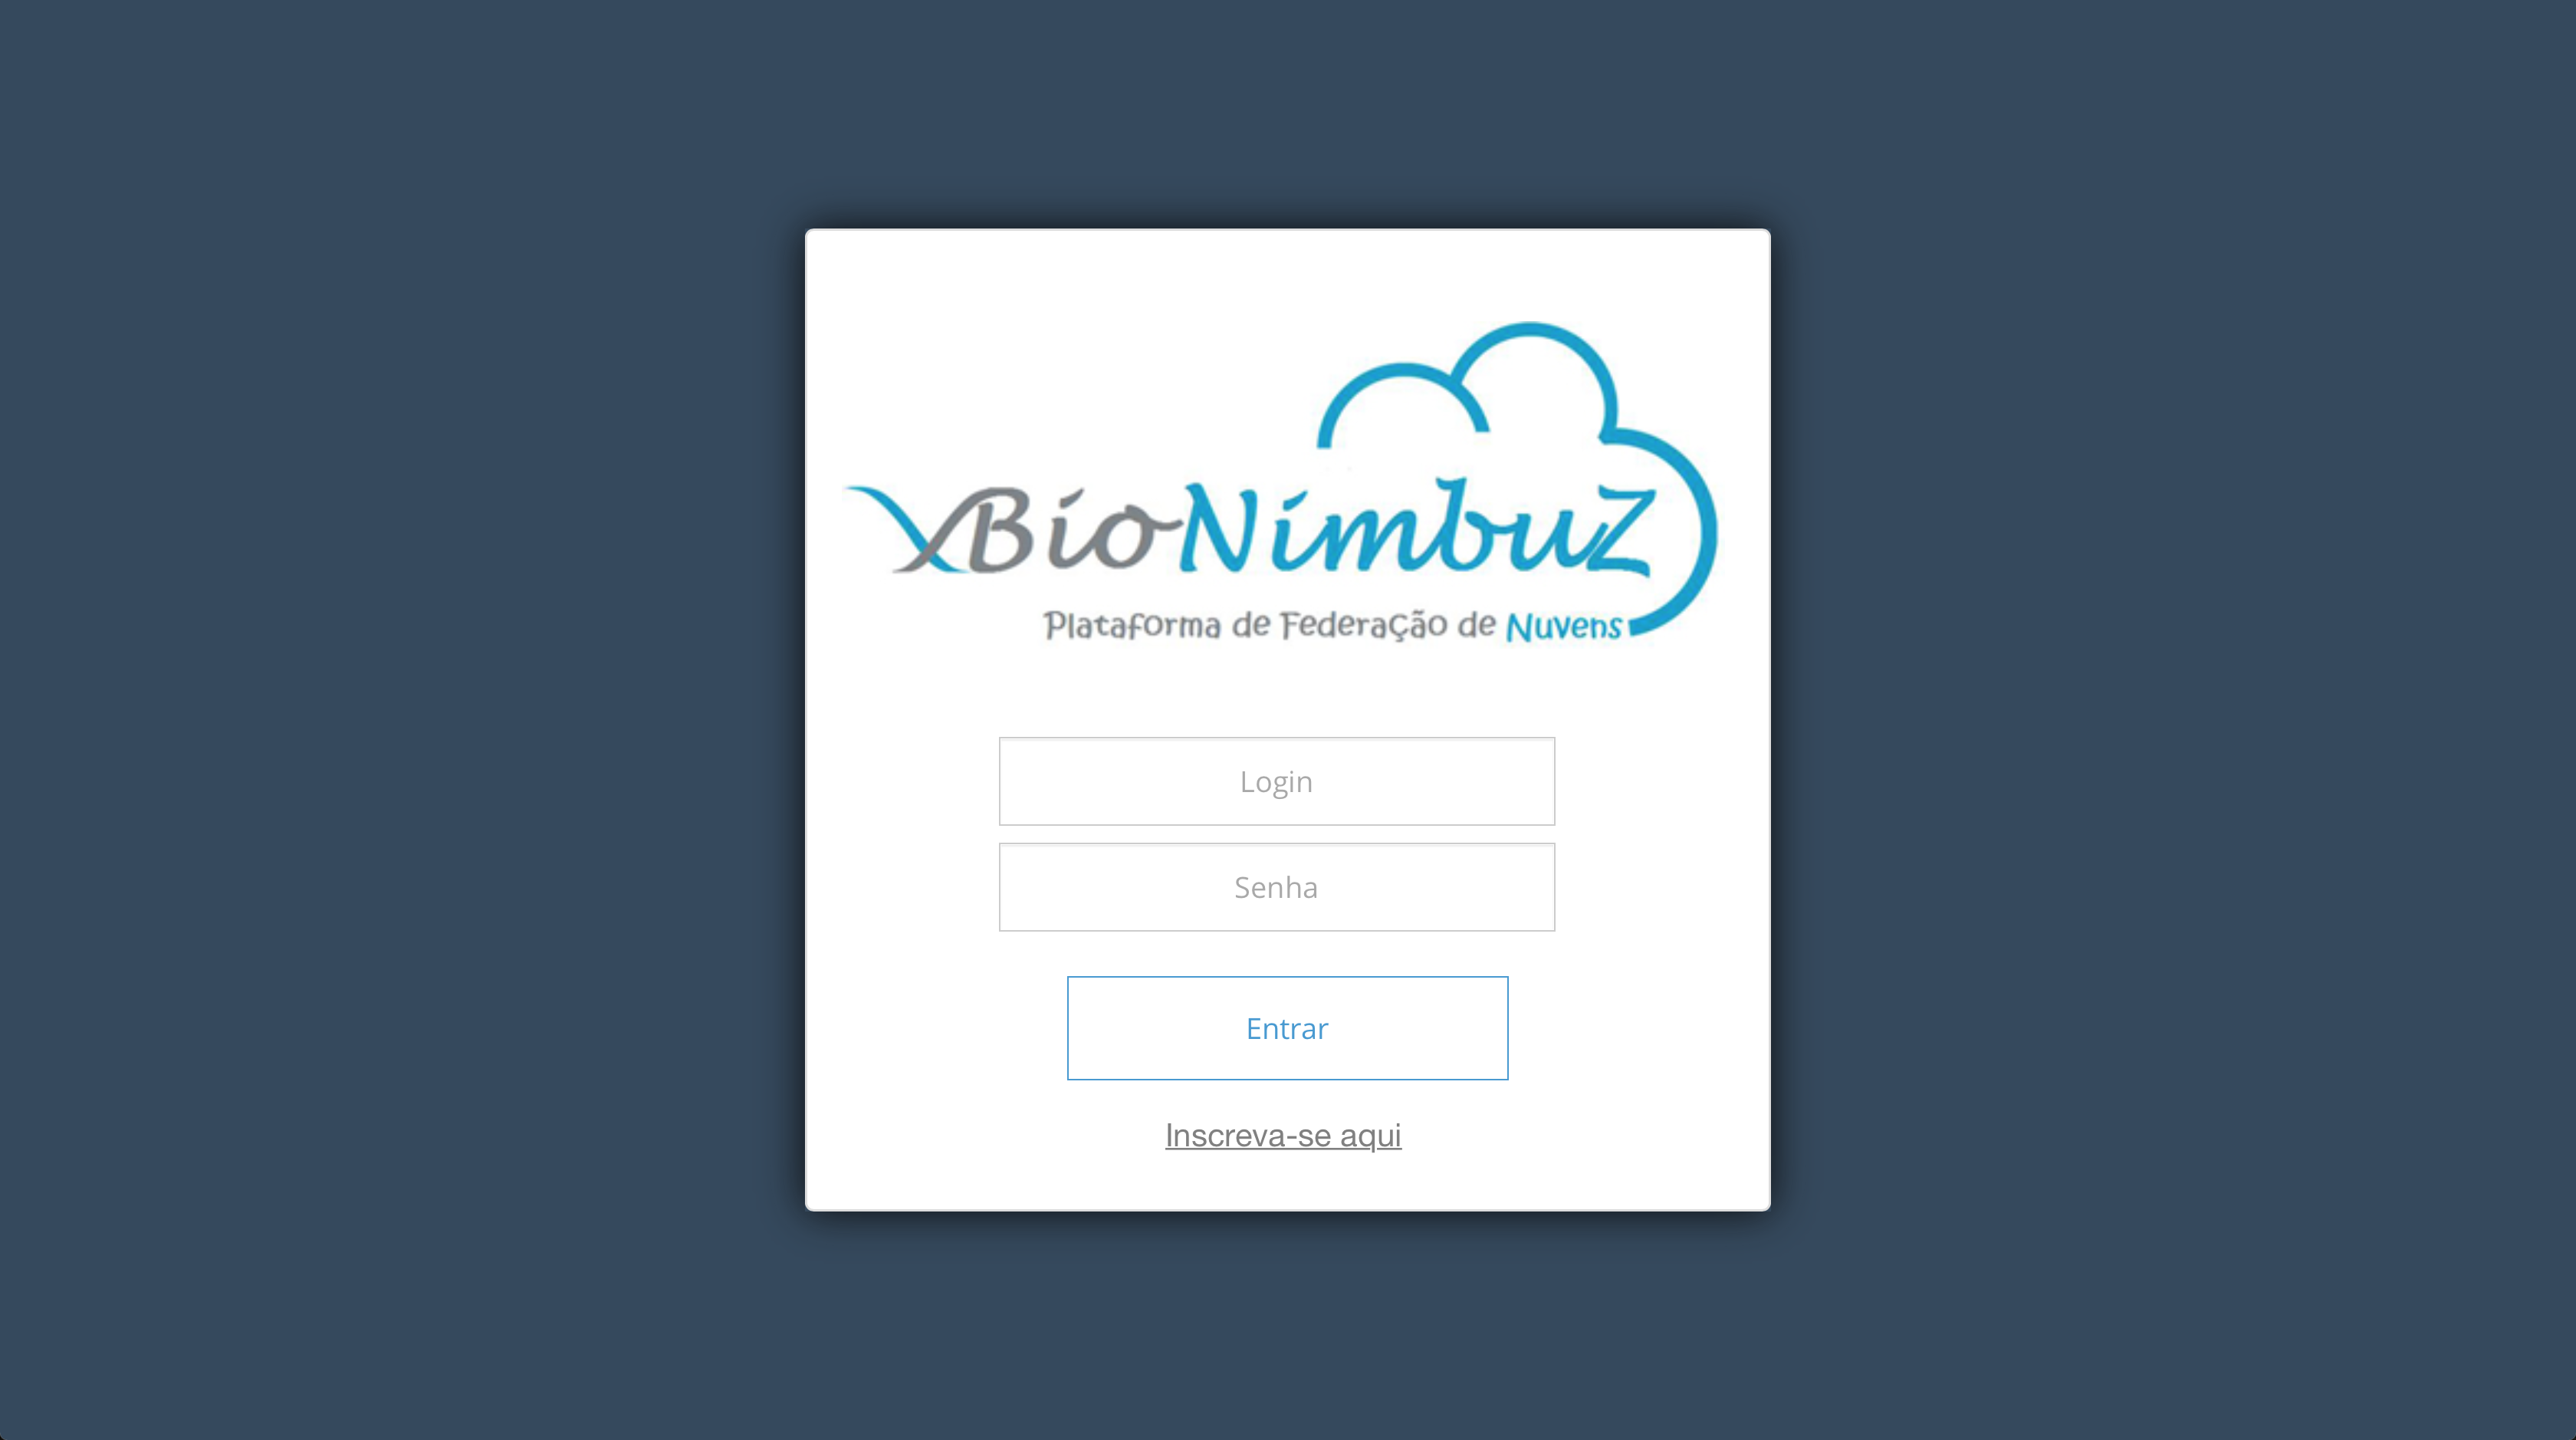
\includegraphics[scale=0.265 ]{tela_login.png}
	\caption{Tela inicial da aplicação \textit{web}.}
	\label{fig:tela_login}
\end{figure}

\noindent
\textbf{Tela de Cadastro} \\

\noindent
Por essa tela, novos usuários se cadastram na plataforma BioNimbuZ, incluindo seus dados, tais como telefone, nome, CPF, etc. A Figura \ref{fig:tela_cadastro} mostra a tela que é apresentada ao usuário.

\begin{figure}[H]
	\centering
	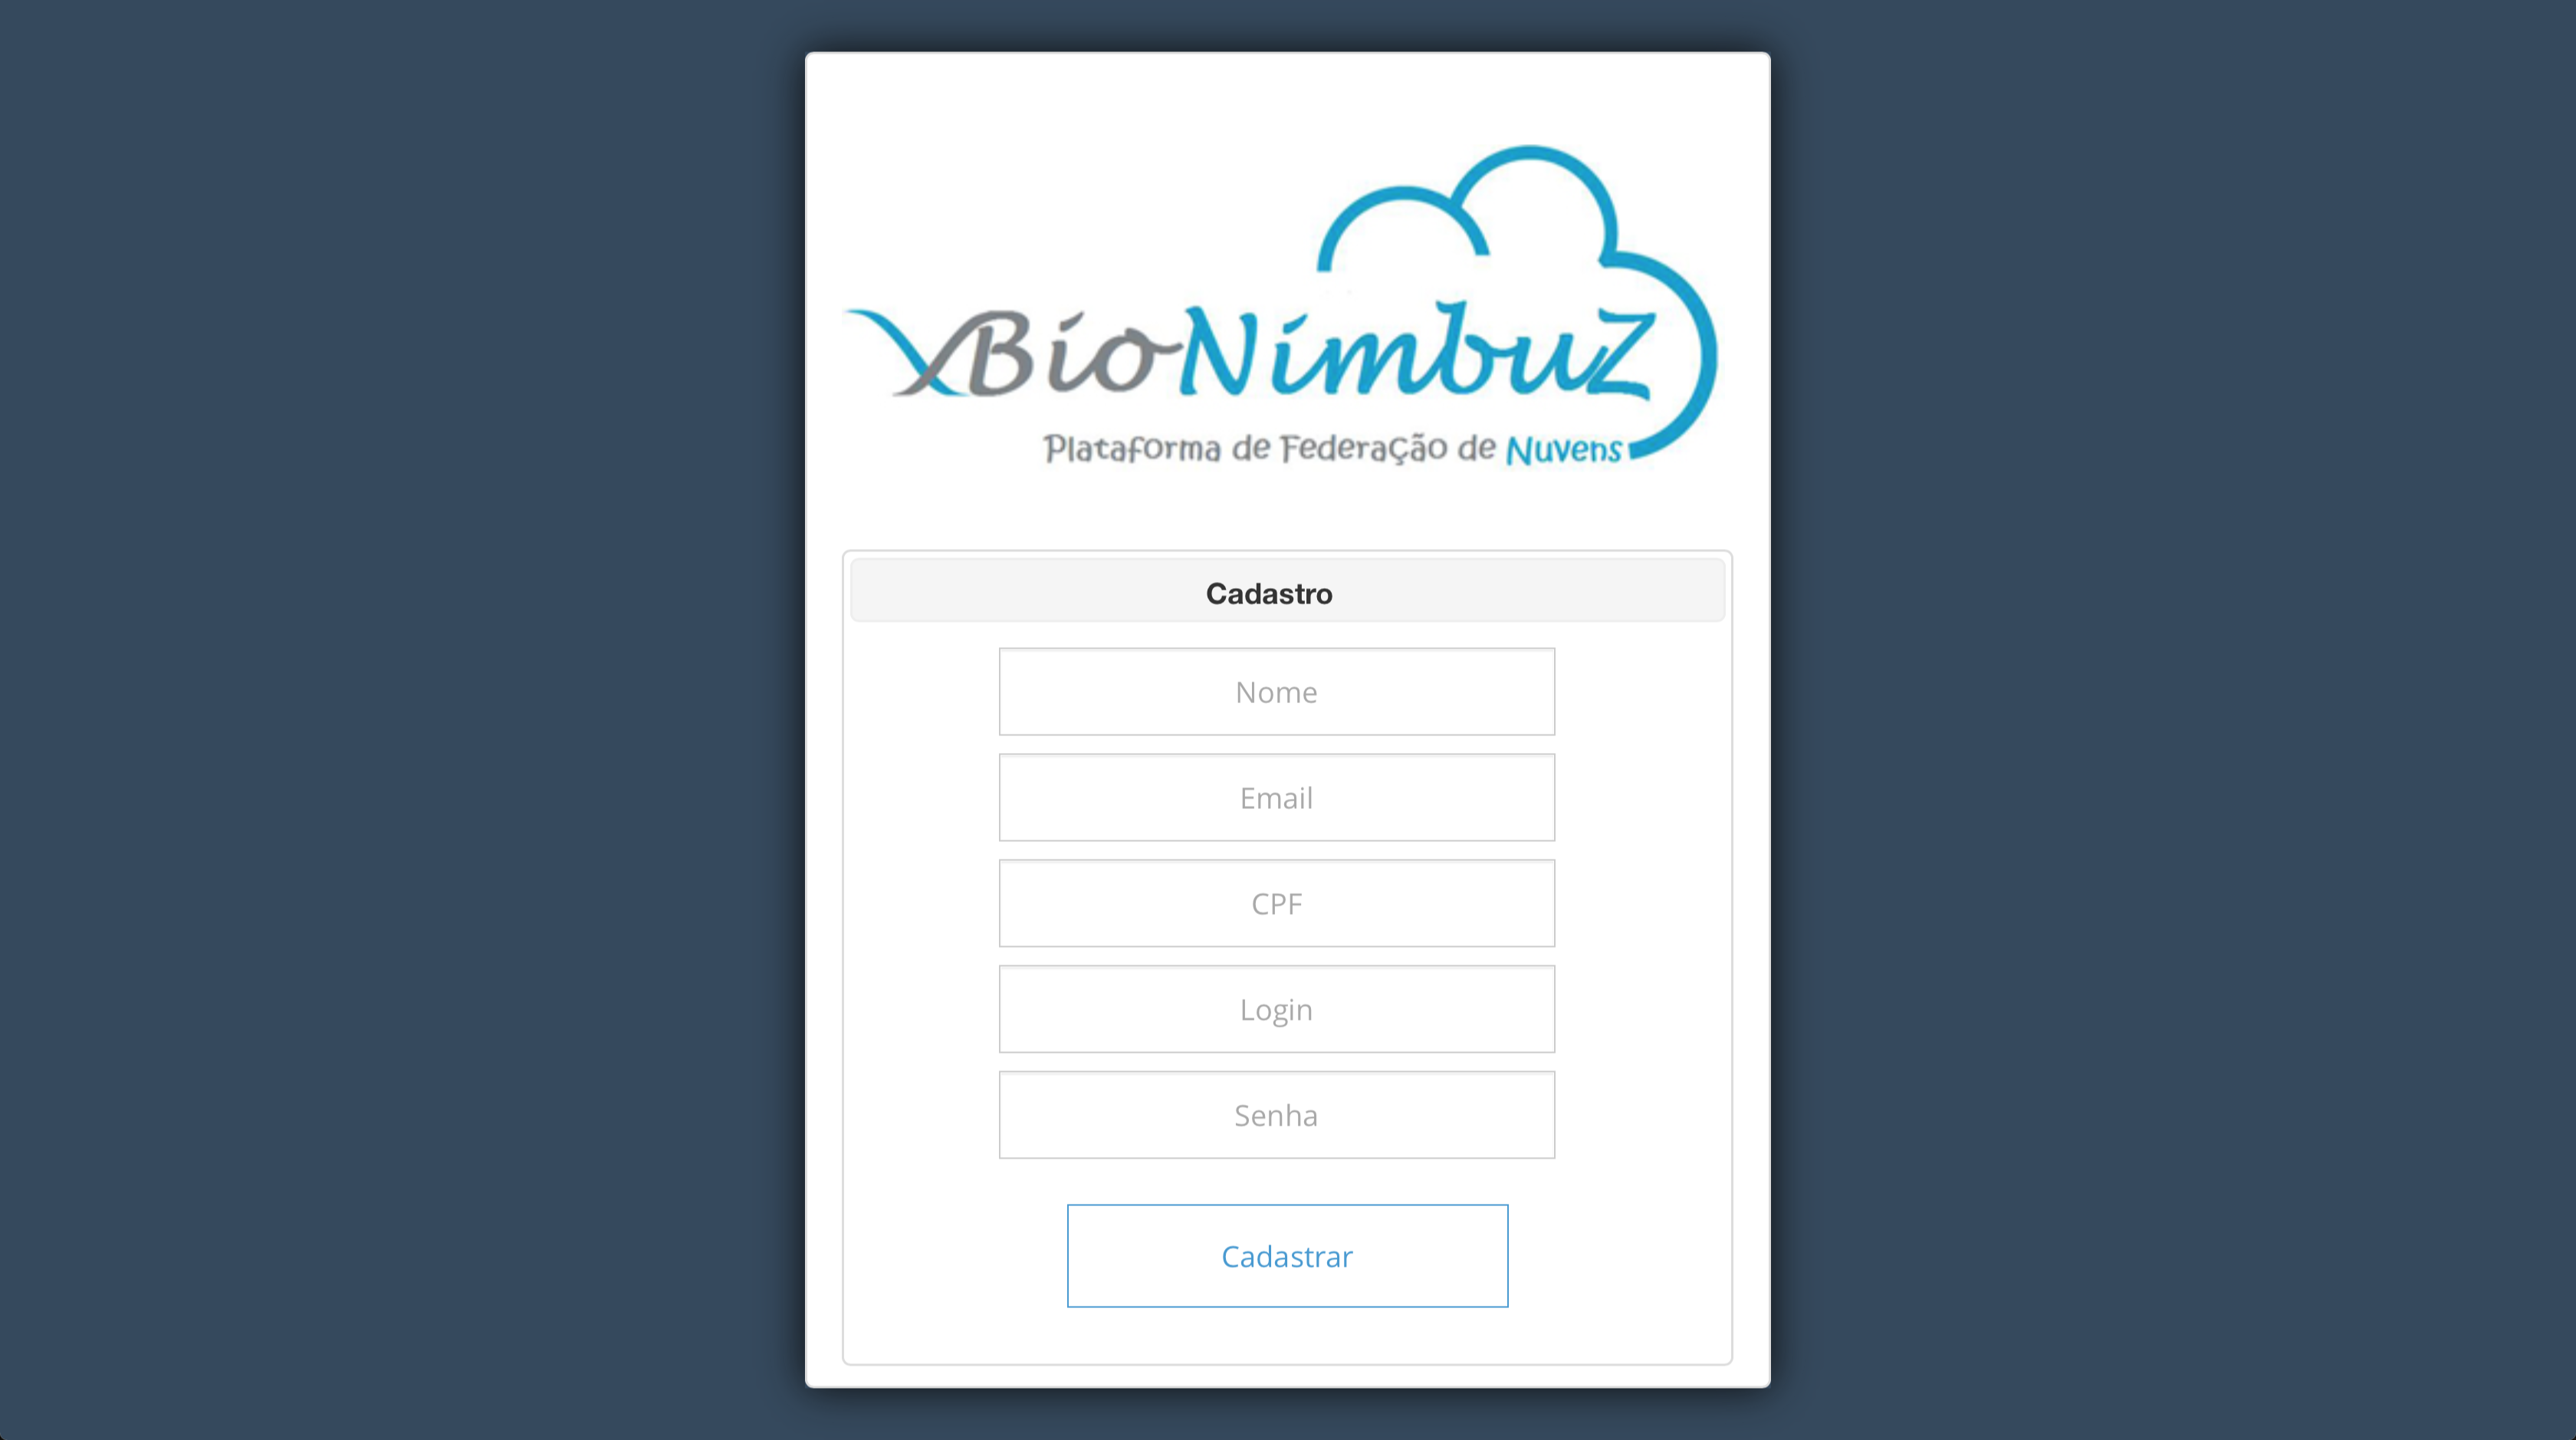
\includegraphics[scale=0.25 ]{tela_cadastro.png}
	\caption{Tela de cadastro de novos usuários.}
	\label{fig:tela_cadastro}
\end{figure}

\noindent
\textbf{\textit{Tela Inicial}} \\

\noindent
Ao realizarem o \textit{login}, os usuários que possuírem acesso ao ambiente \textit{web} visualizarão a tela mostrada na Figura \ref{fig:tela_inicial}. Essa tela dá acesso às opções disponíveis no BioNimbuZ, tais como criar um novo \textit{workflow}, visualizar seu \textit{status}, enviar arquivos para plataforma, etc.

\begin{figure}[H]
	\centering
	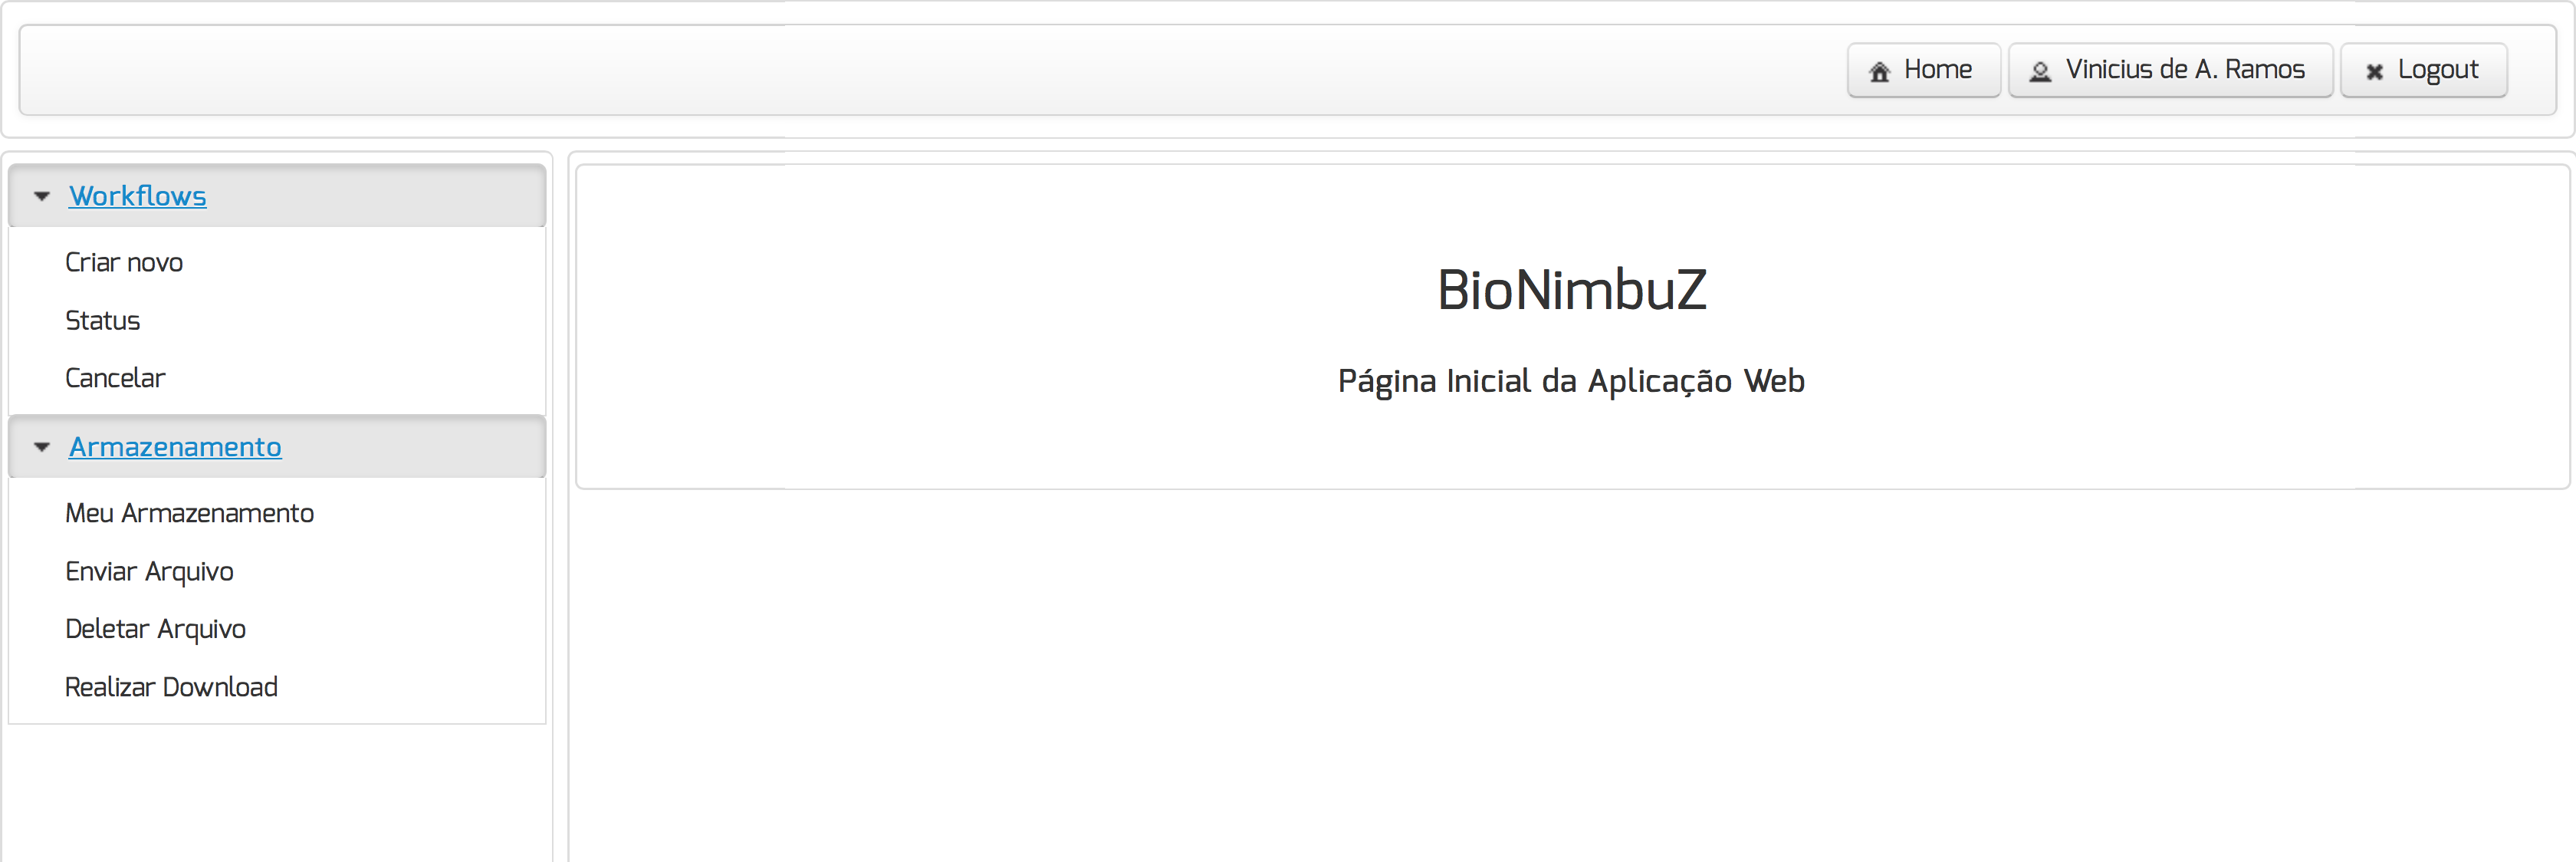
\includegraphics[scale=0.25 ]{tela_inicial.png}
	\caption{Tela inicial da aplicação \textit{web}.}
	\label{fig:tela_inicial}
\end{figure}

\noindent
\textbf{Tela inicial da criação dos \textit{Workflows}} \\

\noindent
Nesta tela, mostrada na Figura \ref{fig:tela_inicial_workflows}, o usuário inicia o projeto de seu \textit{workflow}, podendo escolher entre criar um novo \textit{workflow} ou importar um anteriormente criado. A aplicação \textit{web} possibilita, ao fim do projeto de um \textit{workflow}, exportá-lo. Assim, com esse \textit{workflow} exportado, é possível compartilhá-lo, sendo este a última fase do ciclo de vida de um \textit{workflow} (detalhado no \refCap{capitulo3}).

\begin{figure}[H]
	\centering
	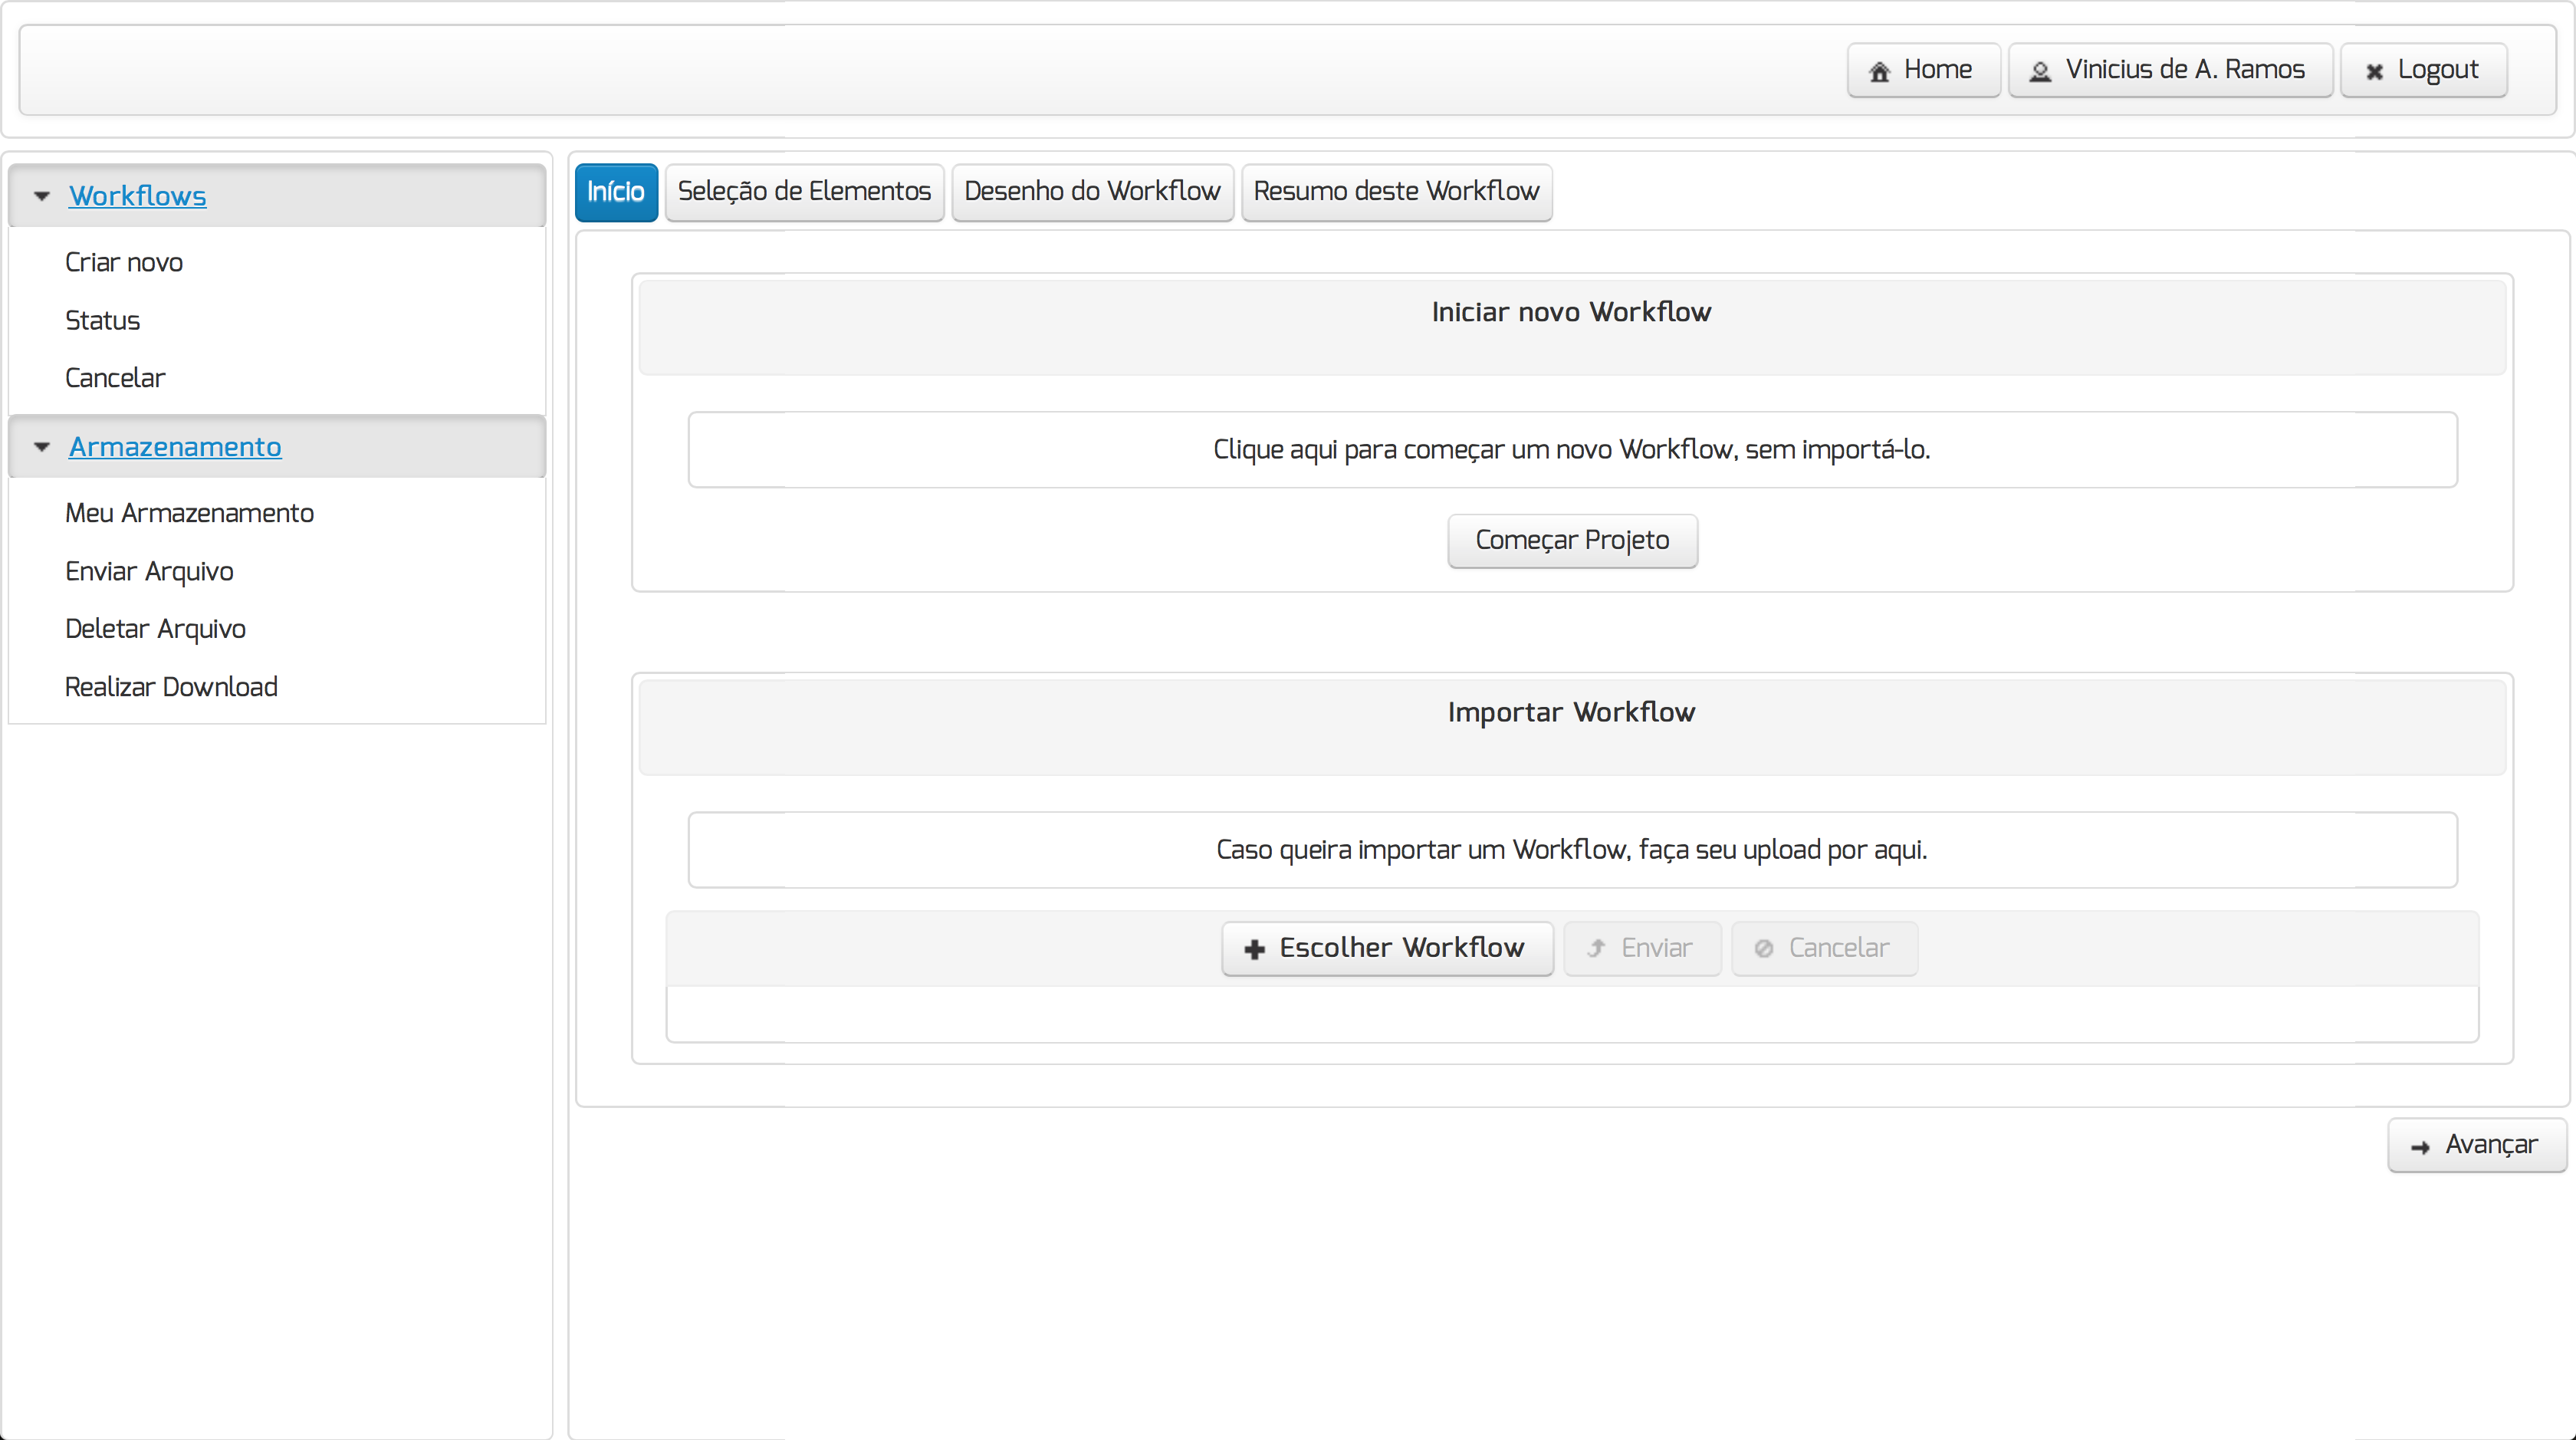
\includegraphics[scale=0.265 ]{tela_inicial_workflows.png}
	\caption{Tela inicial de criação dos \textit{workflows}.}
	\label{fig:tela_inicial_workflows}
\end{figure}

\noindent
\textbf{Tela de seleção de elementos} \\

\noindent
Ao clicar em ''Começar Projeto'', o usuário então é direcionado para a página de seleção de elementos, mostrada na Figura \ref{fig:tela_selecao_elementos}. Nela, o mesmo poderá planejar a execução de seu \textit{workflow}, escolhendo quais elementos irão compor este fluxo. A lista de elementos disponíveis é mantida no núcleo do BioNimbuZ e é enviada à aplicação quando esta é iniciada. À medida que o usuário escolhe os elementos, eles são adicionados na listagem ''Elementos Escolhidos'', podendo o mesmo excluí-los, caso não os queira mais.

\begin{figure}[H]
	\centering
	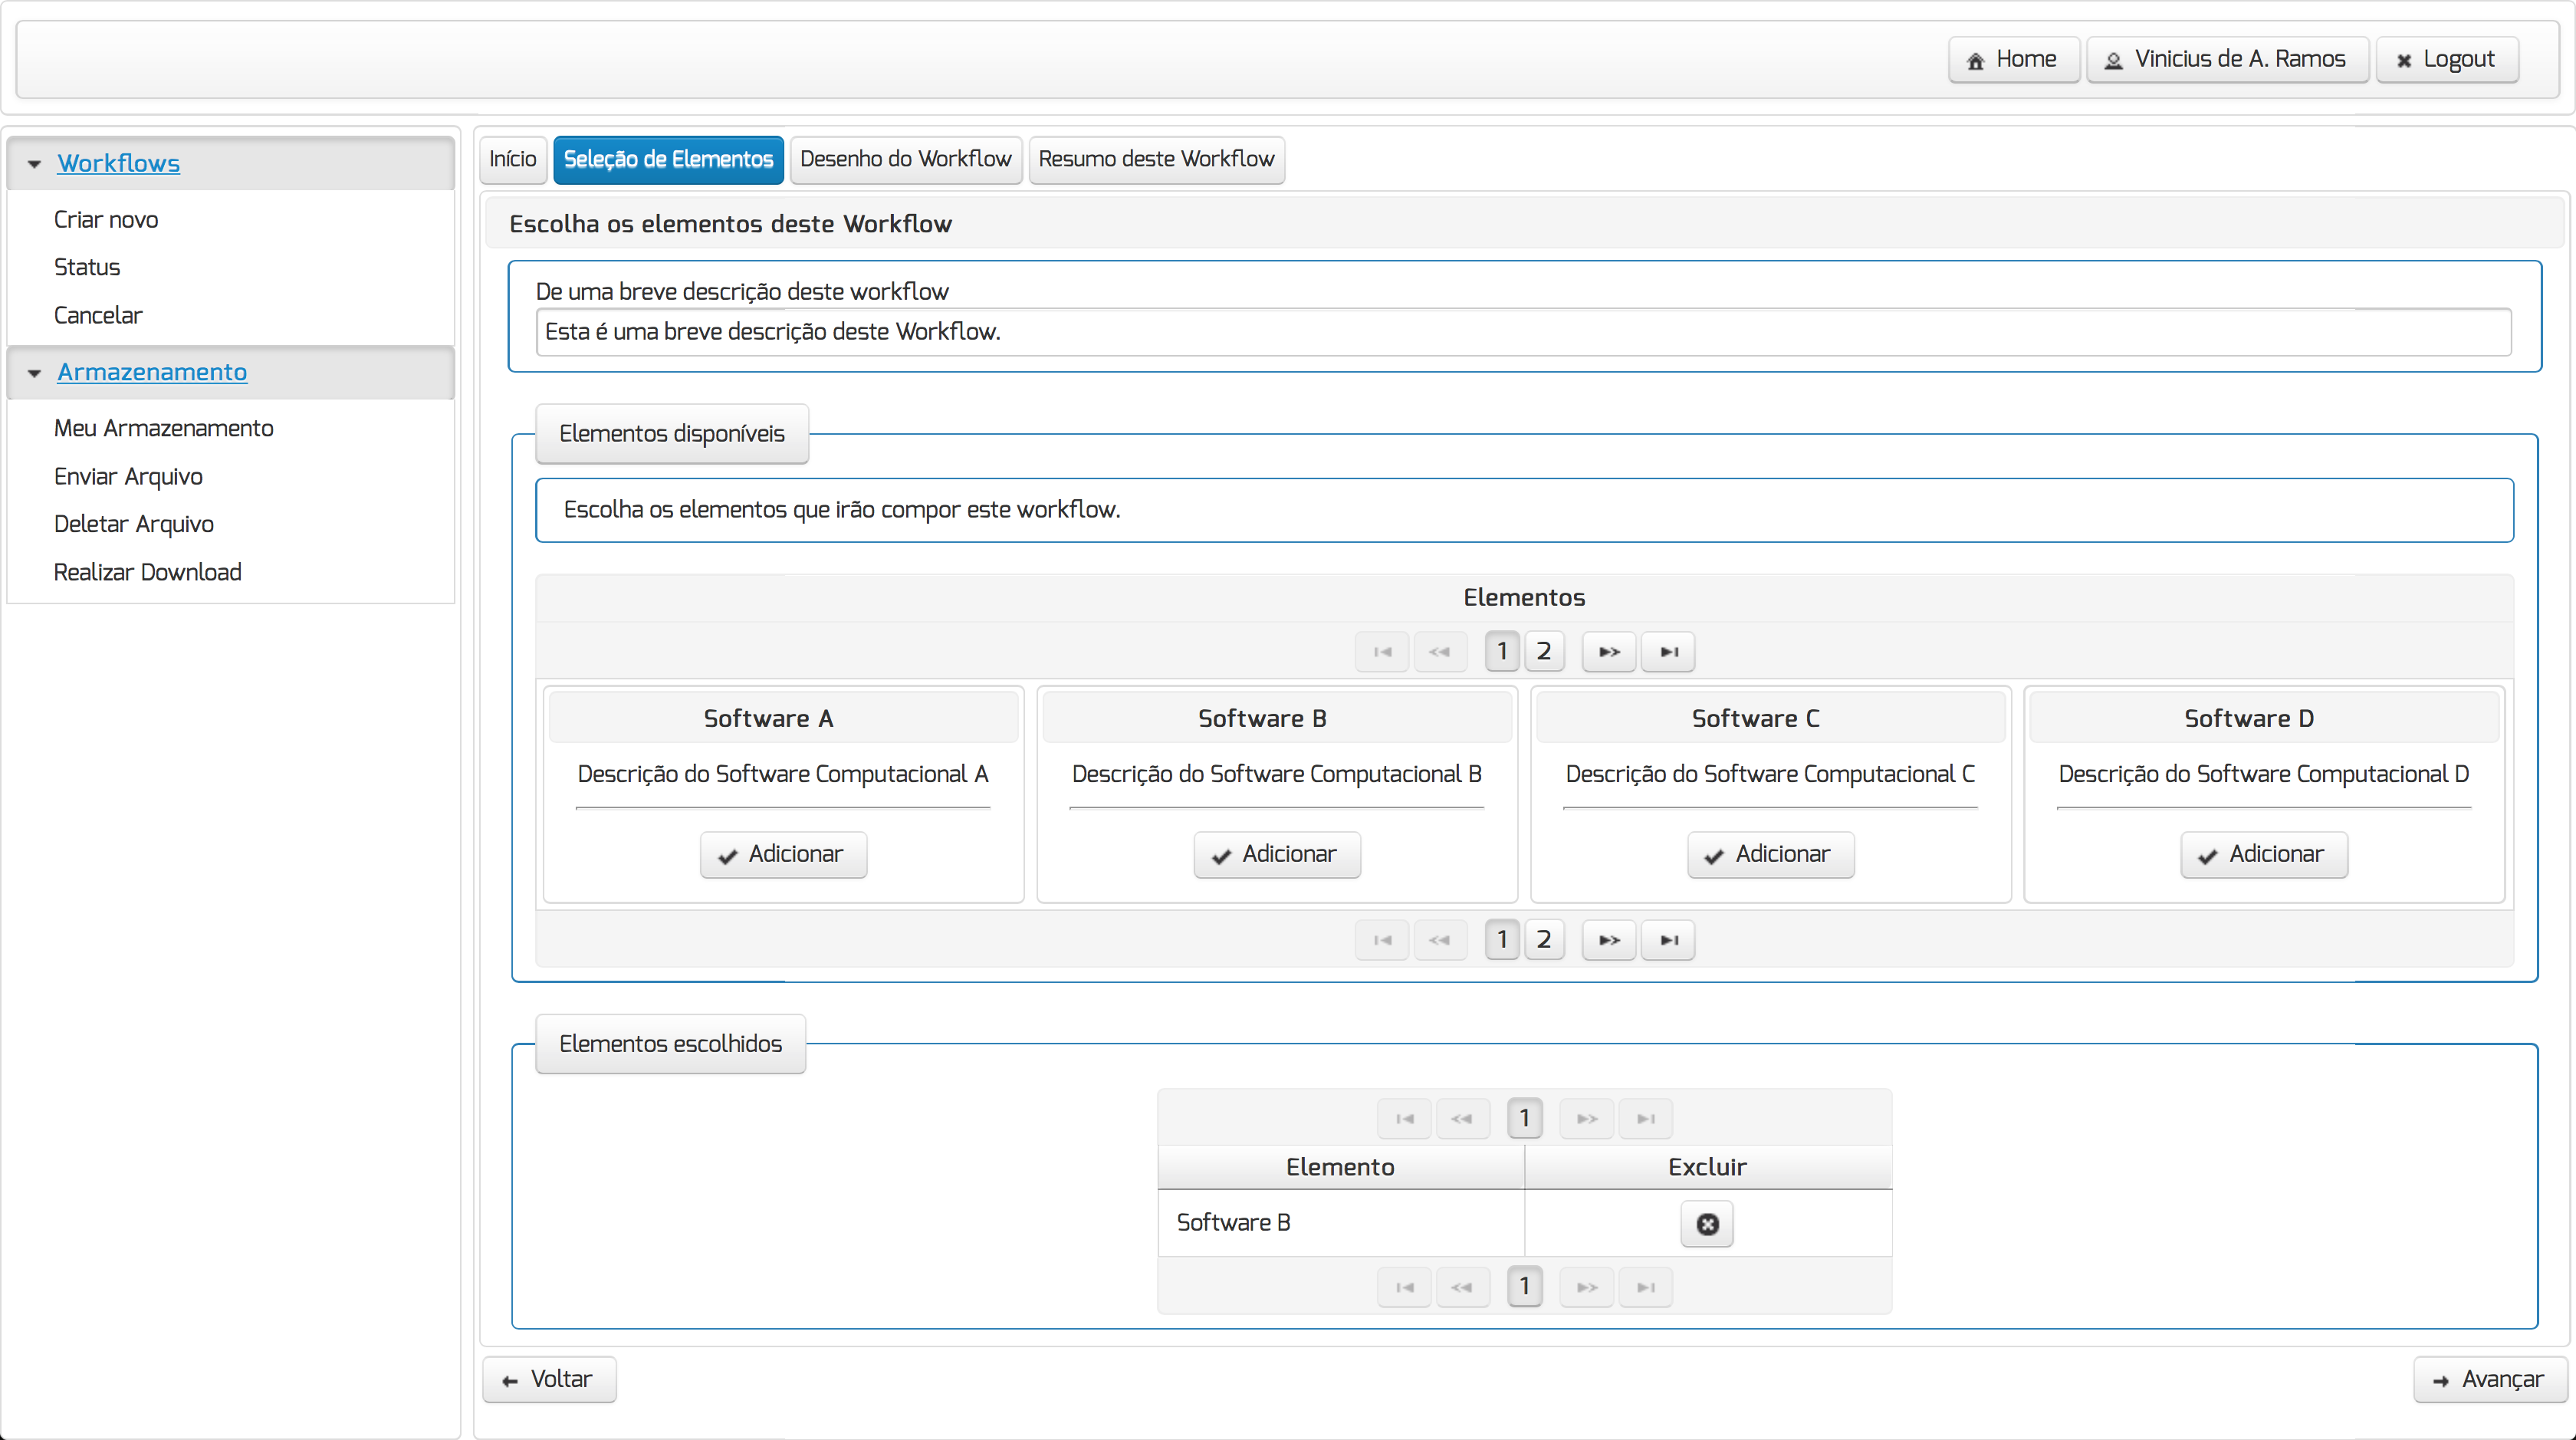
\includegraphics[scale=0.265 ]{tela_selecao_elementos.png}
	\caption{Tela utilizada para selecionar elementos que irão compôr o \textit{workflow}.}
	\label{fig:tela_selecao_elementos}
\end{figure}

\noindent
\textbf{Tela de \textit{design} do \textit{workflow}} \\

\noindent
Com os elementos definidos na tela anterior (Figura \ref{fig:tela_selecao_elementos}), o usuário é redirecionado para a tela seguinte, passando para a fase de \textit{design} do \textit{workflow}. Nela, são apresentados os elementos escolhidos pelo usuário dispostos de maneira gráfica, conforme mostra a \ref{fig:tela_design_workflow}.

\begin{figure}[H]
	\centering
	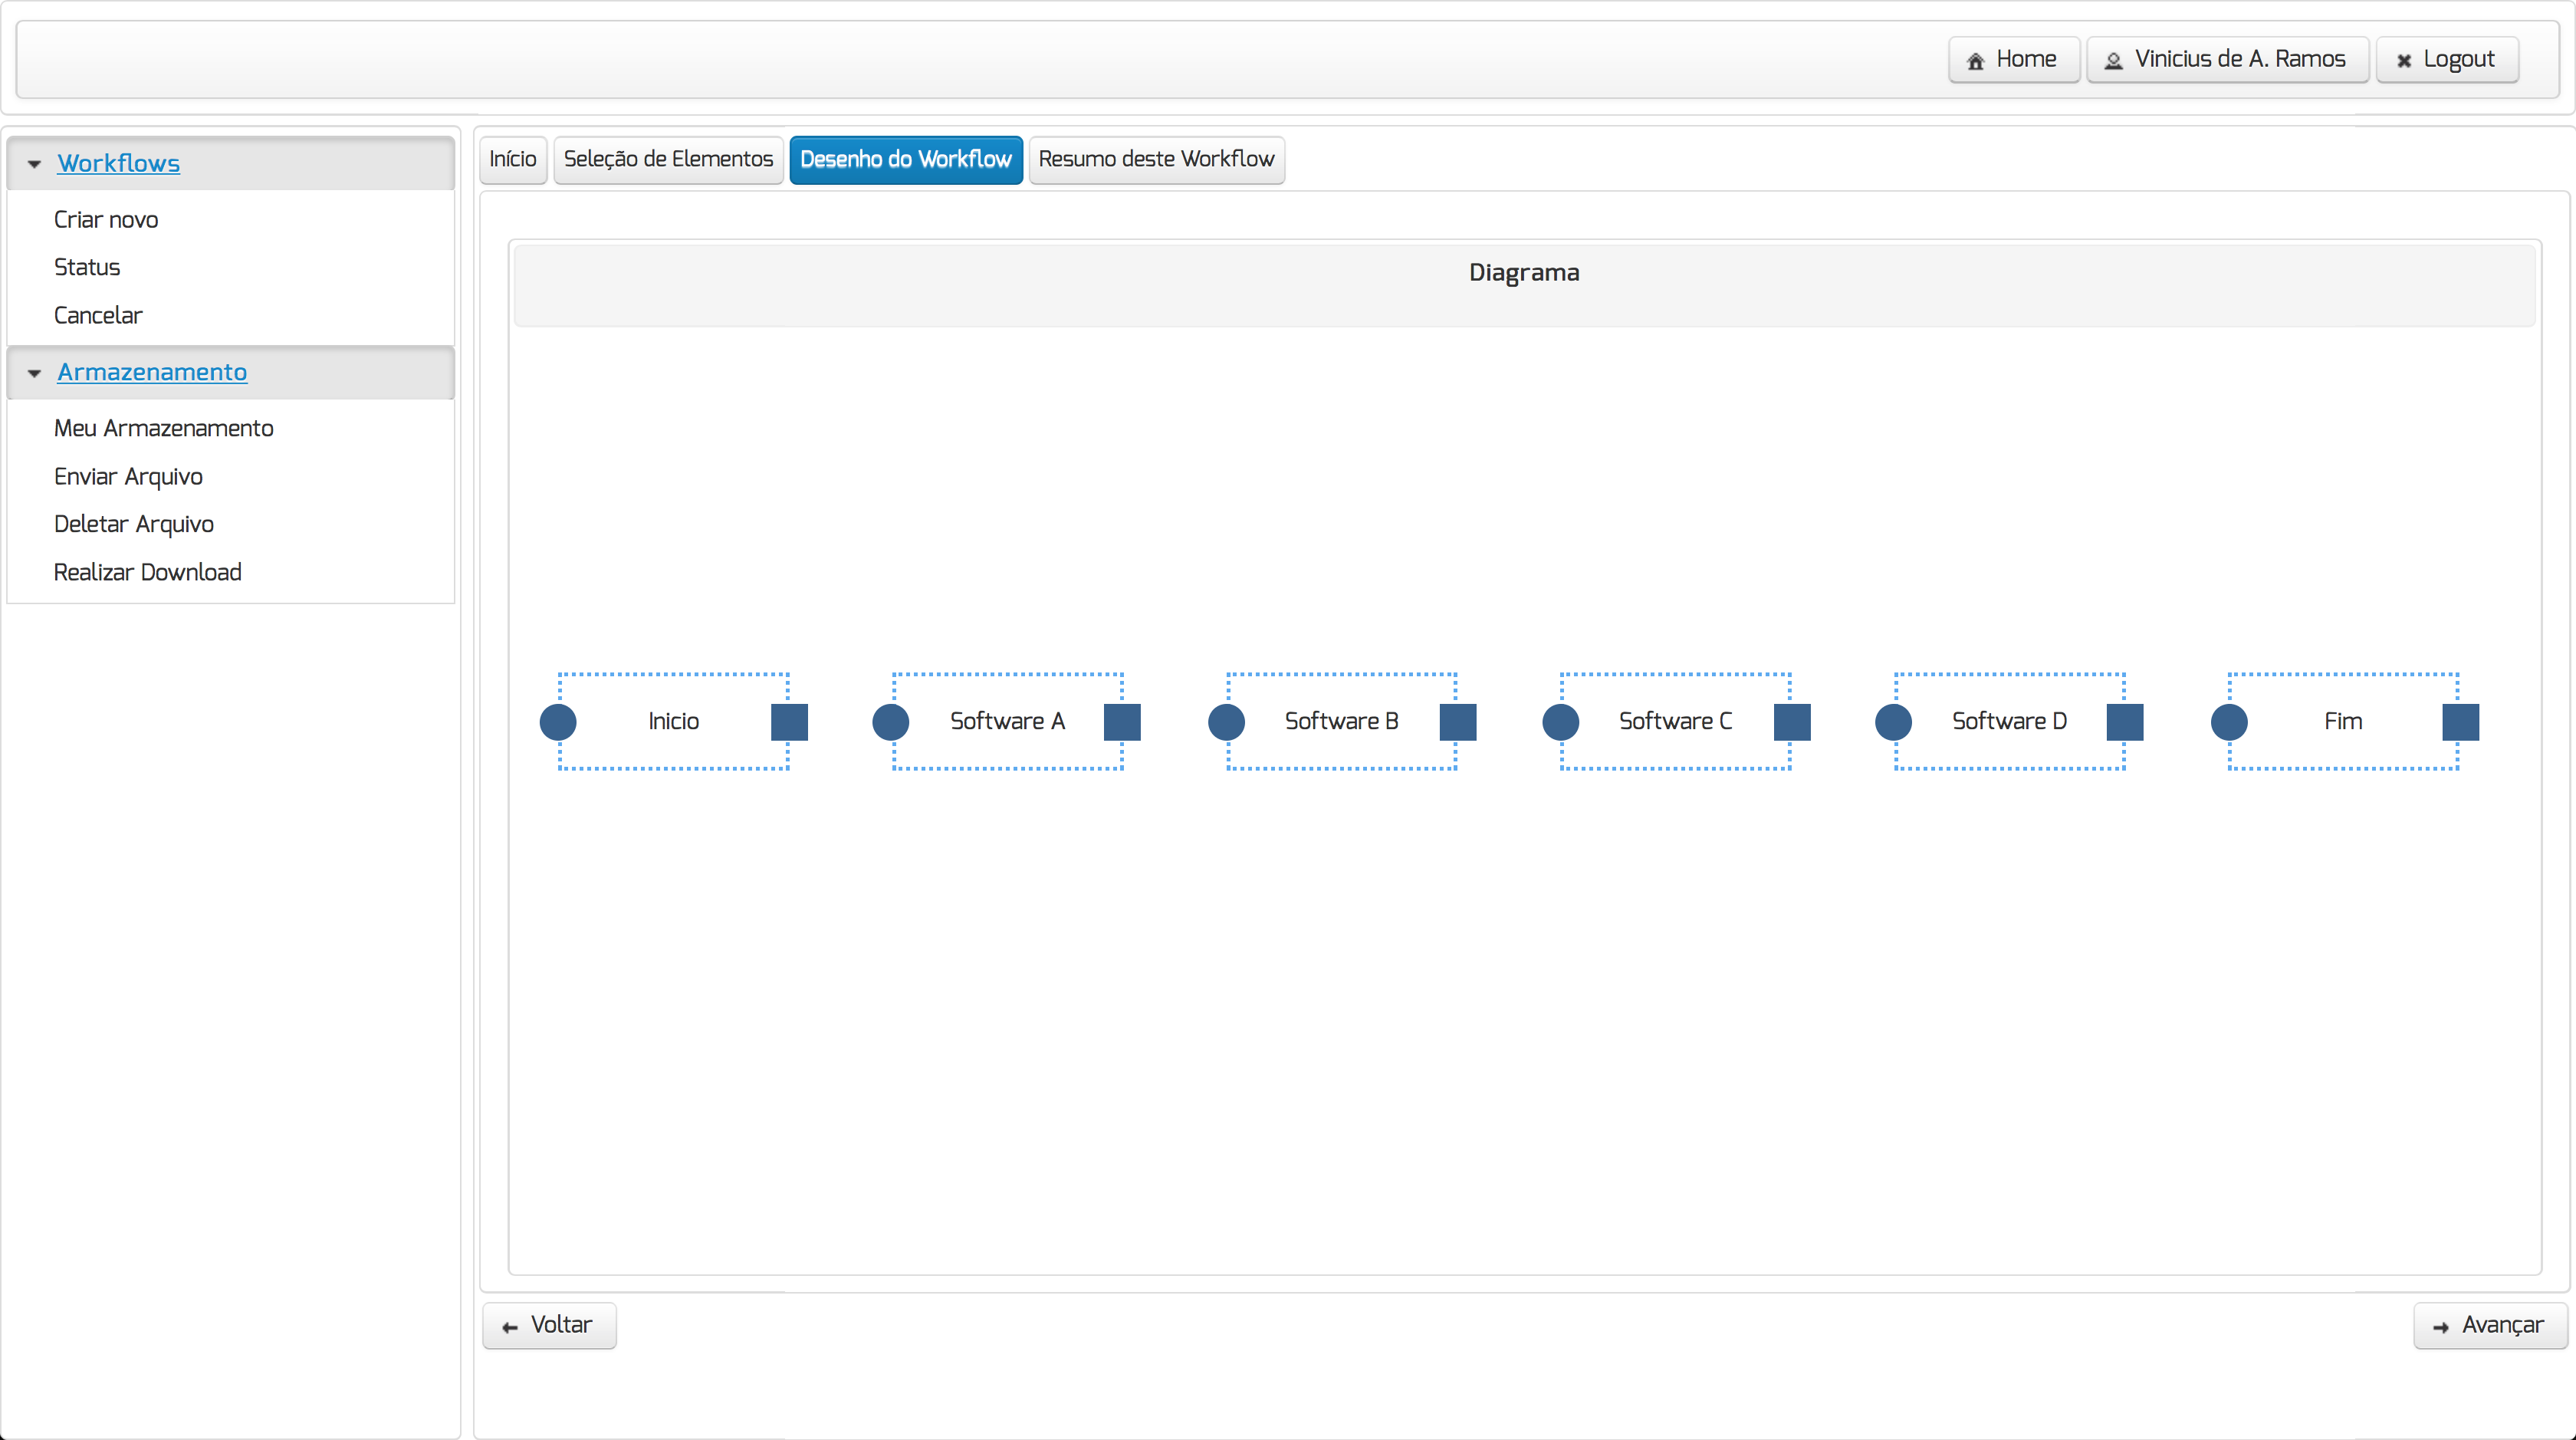
\includegraphics[scale=0.265 ]{tela_design_workflow.png}
	\caption{Nesta tela o usuário compõe o fluxo de seu \textit{workflow}.}
	\label{fig:tela_design_workflow}
\end{figure}

Com isso, o usuário pode definir as dependências de cada elemento, arrastando os pontos de ligação, definir suas entradas (arquivos enviados ou uma URL que contenha o caminho para realizar o download do arquivo para a plataforma BioNimbuZ), definir os parâmetros de execução (como argumentos daquele componente) ou apenas sinalizar que a entrada de um determinado elemento será a saída de outro. Para isso, ao se conectar dois elementos, é mostrada uma caixa de diálogo pedindo estes dados (Figura 5.9).

\begin{figure}[H]
	\centering
	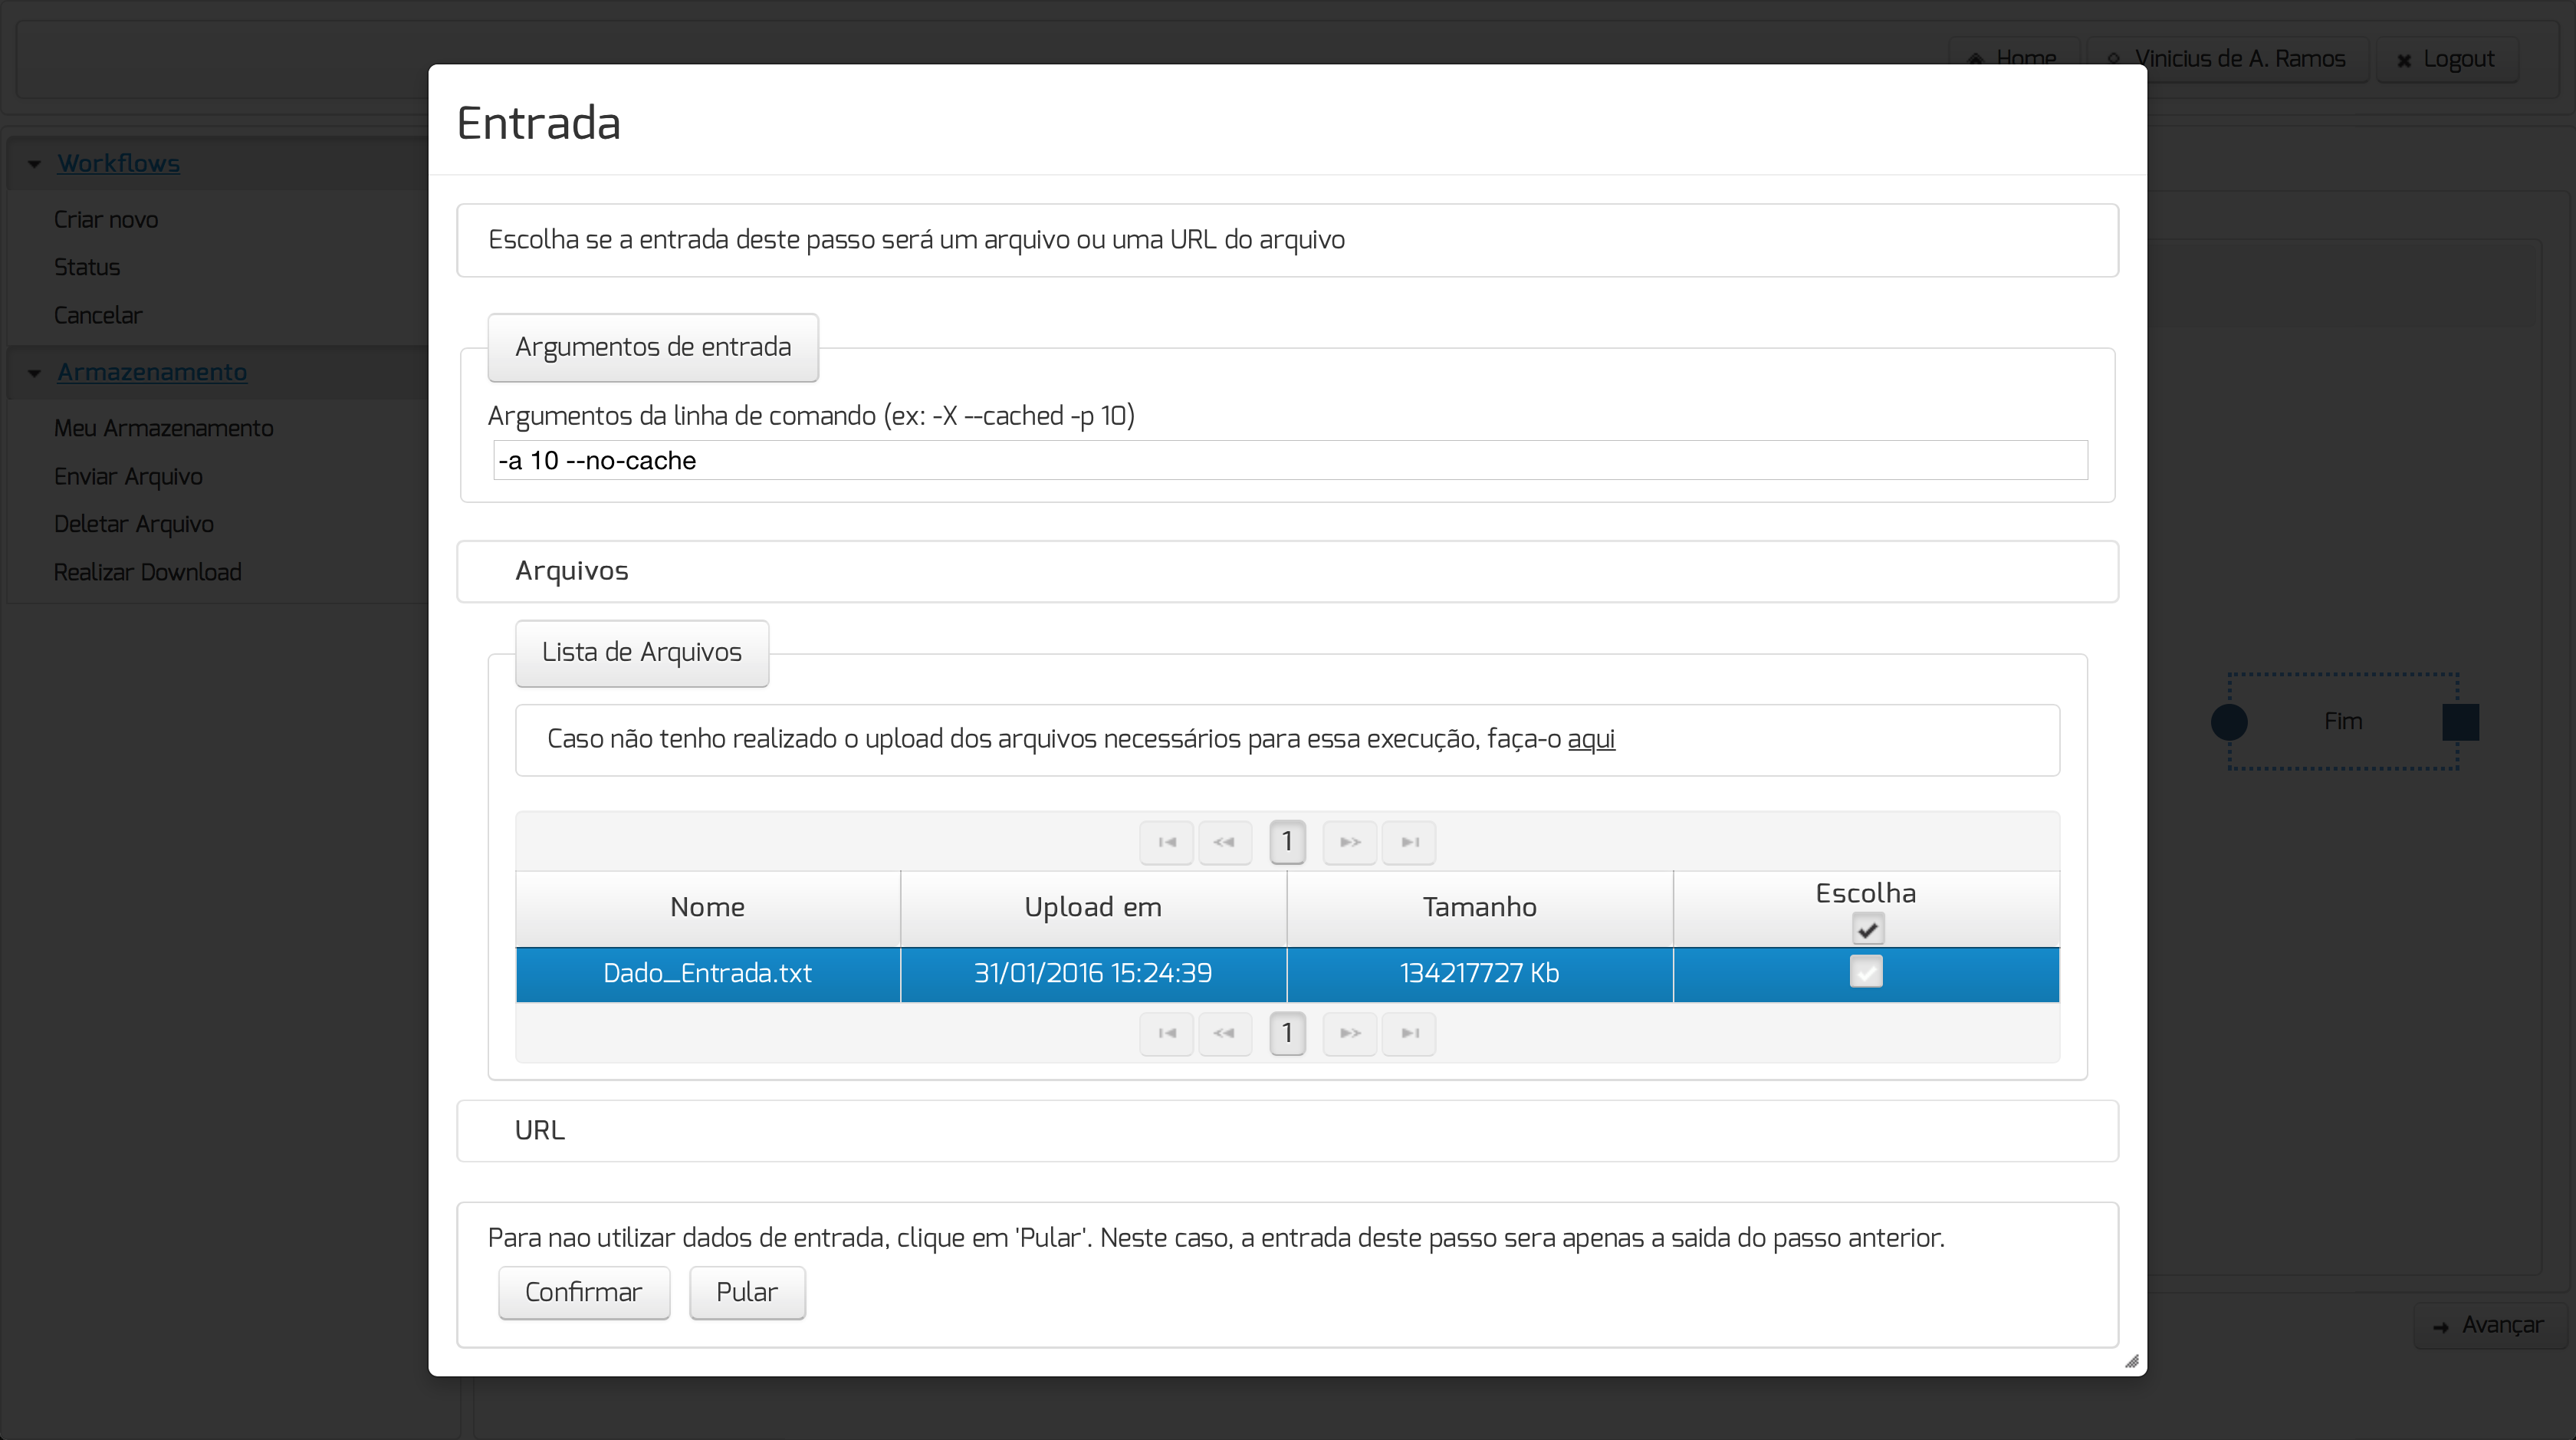
\includegraphics[scale=0.265 ]{tela_definicao_entrada.png}
	\caption{Nesta tela o usuário define parâmetros de execução de um elemento do \textit{workflow}.}
	\label{fig:tela_definicao_entrada}
\end{figure}

\noindent
\textbf{Tela de Confirmação} \\

\noindent
Com todos os elementos escolhidos e com suas dependências (entrada, saída e parâmetros de execução) satisfeitas, é apresentada uma tela de confimação (Figura \ref{fig:tela_final_workflow}), em que o usuário pode confirmar os dados daquele \textit{workflow} e submetê-lo à execução, ou pode apenas realizar o \textit{download} do arquivo \textbf{\textit{.flow}} (representação do objeto Java contendo os dados de um \textit{workflow}). De posse deste arquivo, o usuário pode importá-lo em outro momento para, por exemplo, finalizá-lo, ou também pode compartilhar este arquivo com outros usuários do sistema, para que outros tenham acesso ao seu trabalho.

\begin{figure}[H]
	\centering
	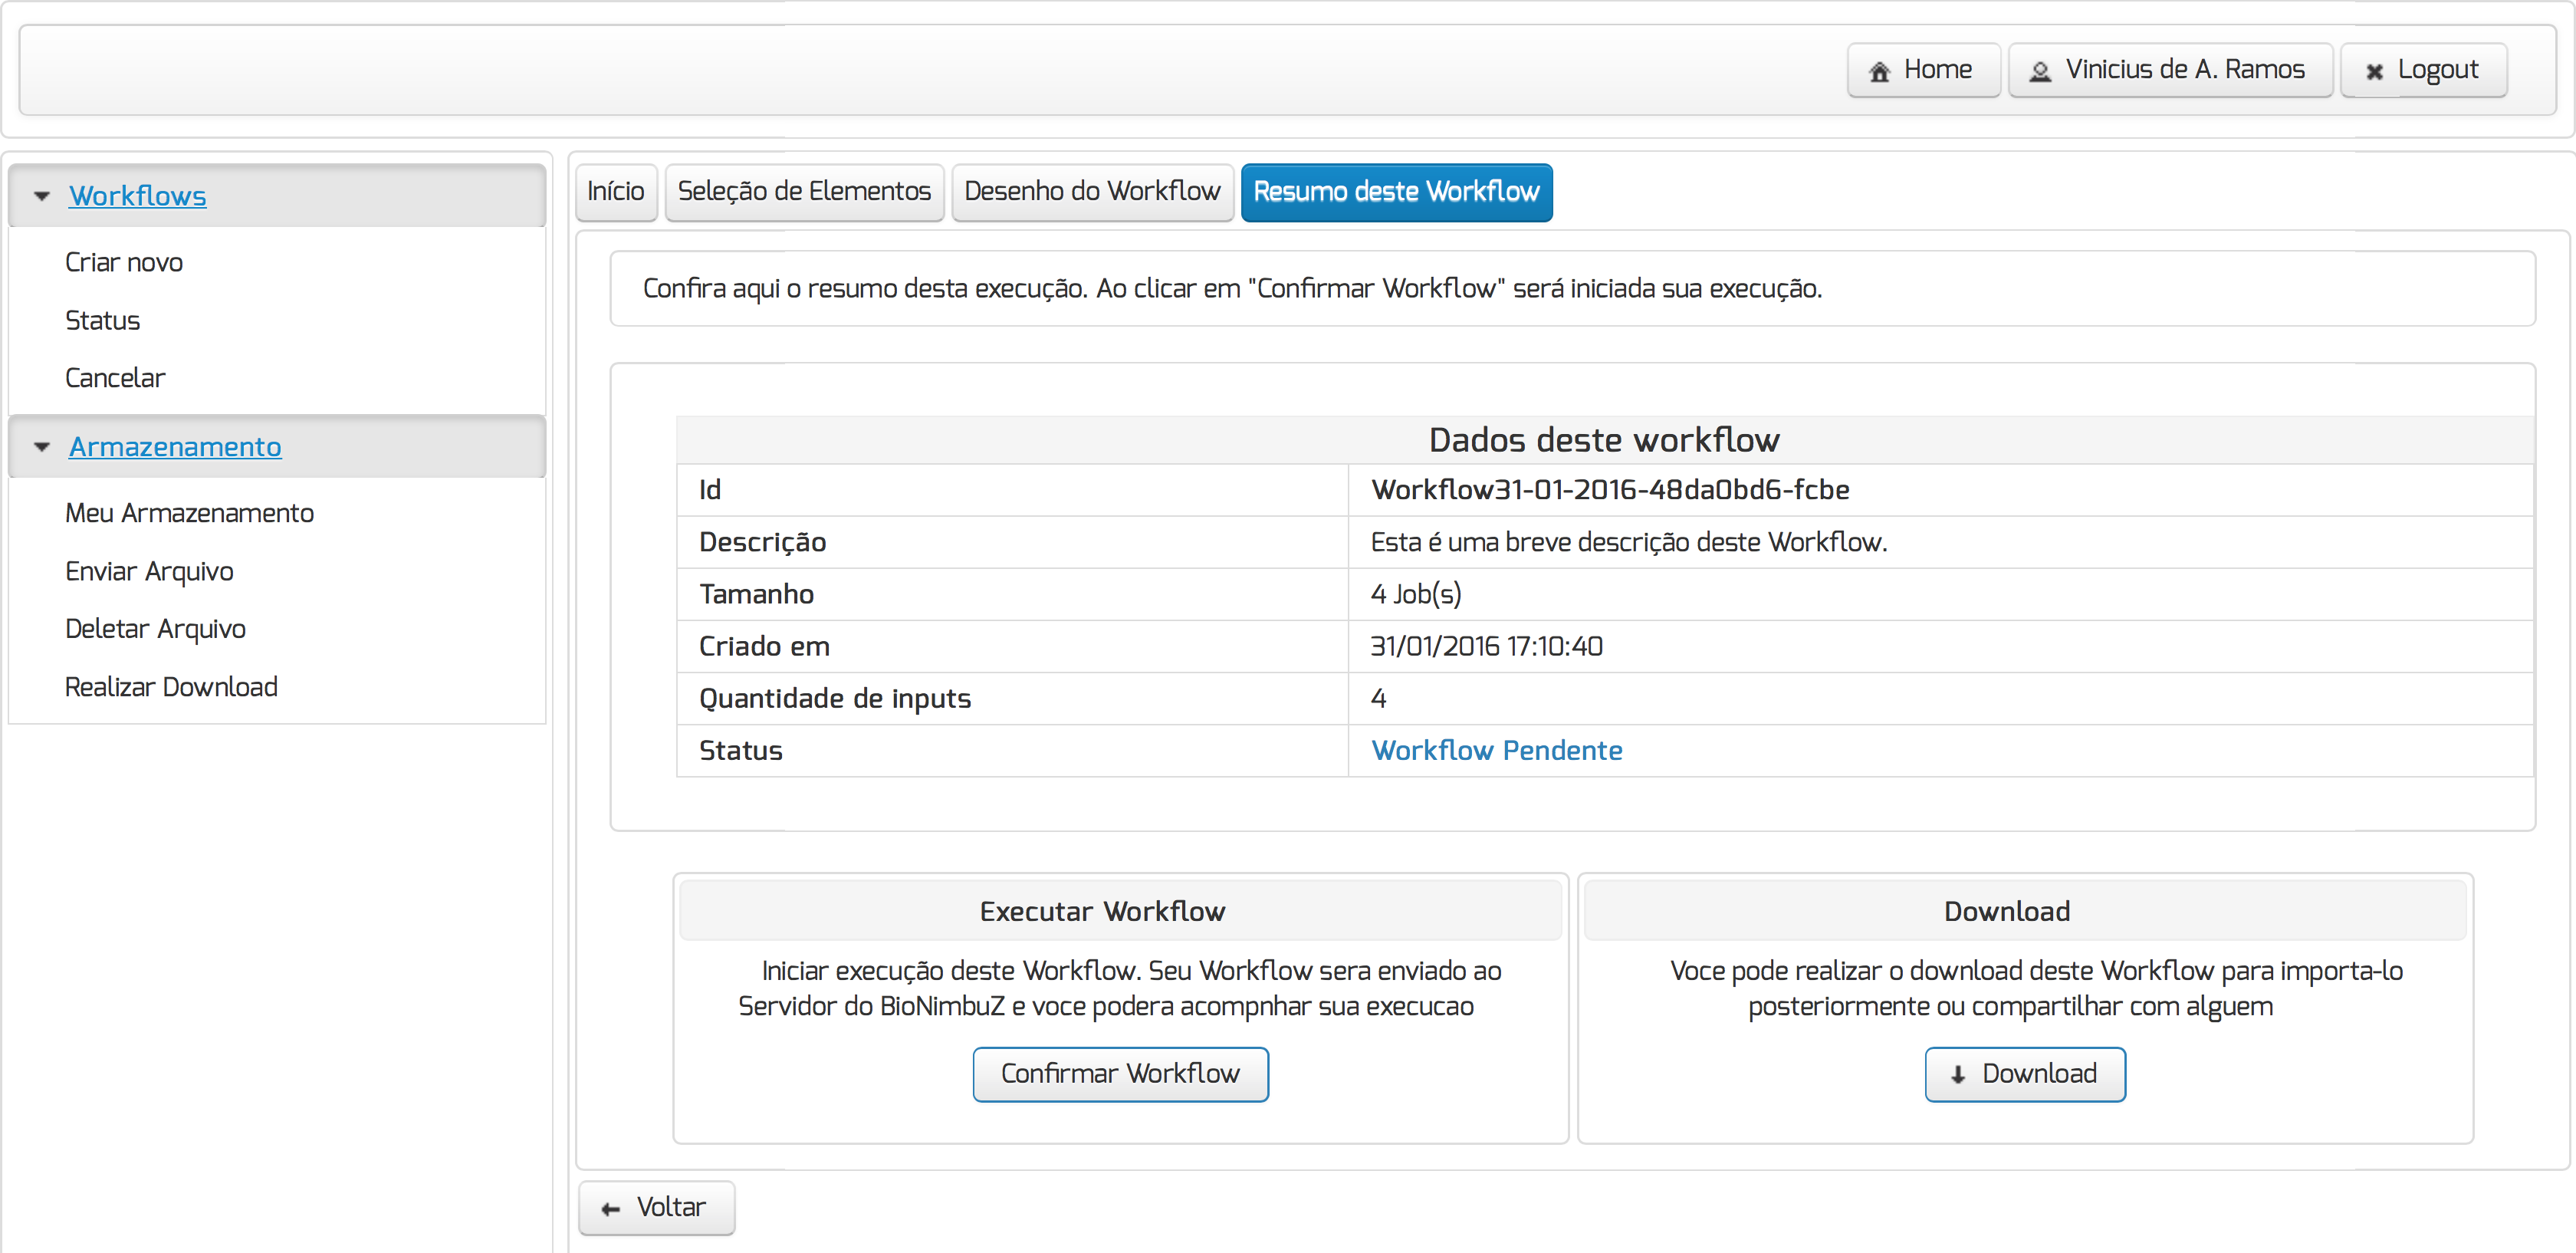
\includegraphics[scale=0.265 ]{tela_final_workflow.png}
	\caption{Tela final da composição do \textit{workflow}.}
	\label{fig:tela_final_workflow}
\end{figure}

\noindent
\textbf{Tela de \textit{status} do \textit{workflow}} \\

\noindent
A partir do momento que o usuário escolheu submeter o \textit{workflow} à plataforma BioNimbuZ, ele pode visualizar o estado de sua execução na tela de \textit{status}, apresentada na Figura \ref{tela_status_workflow}. 

\begin{figure}[H]
	\centering
	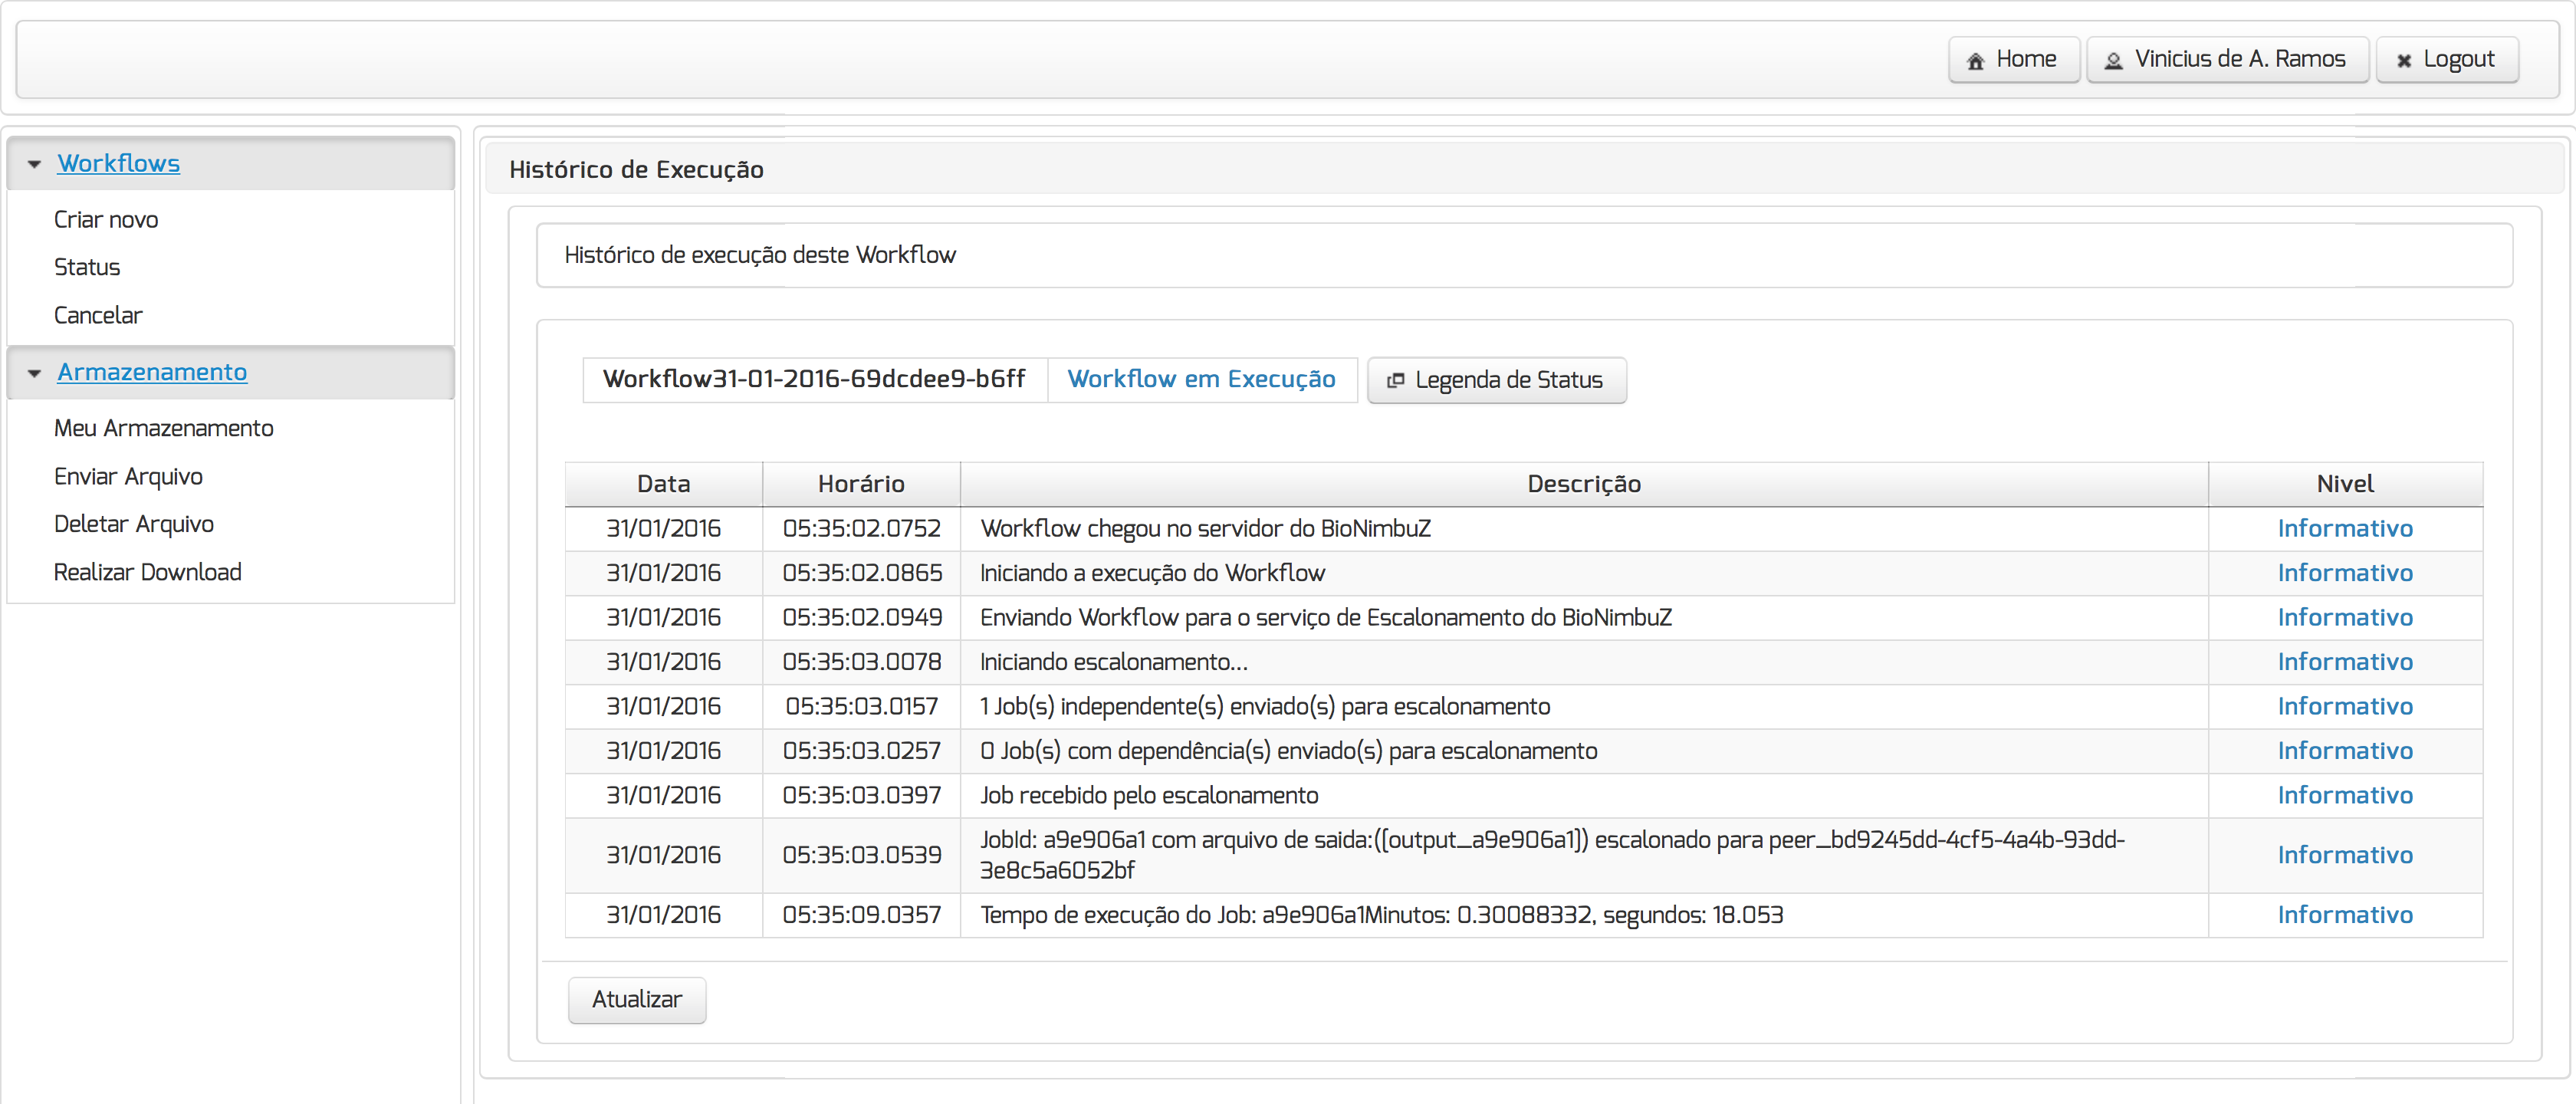
\includegraphics[scale=0.265 ]{tela_status_workflow.png}
	\caption{Tela final da composição do \textit{workflow}.}
	\label{fig:tela_status_workflow}
\end{figure}

Os possíveis estados de um \textit{workflow} estão retratados na Tabela \ref{tab:tabela_status_workflow}.


\begin{table}[H]
\centering
\resizebox{\textwidth}{!}{%
\begin{tabular}{||c|c|c||}
\hline
\large{\textbf{\textit{Status}}} & \large{\textbf{Nível}} & \large{\textbf{Descrição}} \\
\hline
\hline
\multicolumn{1}{||l|}{{\color[HTML]{7F8C8D} \textbf{\textit{Workflow} Pausado}}}                & \multicolumn{1}{l|}{\texttt{Informativo}} & \multicolumn{1}{l||}{Foi requisitada a pausa na execução do \textit{Workflow}.}               \\ 
\hline
\multicolumn{1}{||l|}{{\color[HTML]{2980B9} \textbf{\textit{Workflow} Pendente}}}               & \multicolumn{1}{l|}{\texttt{Informativo}} & \multicolumn{1}{l||}{Seu \textit{Workflow} está agurdando execução pelo BioNimbuZ.}           \\ 
\hline
\multicolumn{1}{||l|}{{\color[HTML]{2980B9} \textbf{\textit{Workflow} em Execução}}}            & \multicolumn{1}{l|}{\texttt{Informativo}} & \multicolumn{1}{l||}{O \textit{Workflow} está em plena execução.}                             \\ 
\hline
\multicolumn{1}{||l|}{{\color[HTML]{27AE60} \textbf{\textit{Workflow} Finalizado com Sucesso}}} & \multicolumn{1}{l|}{\texttt{Informativo}} & \multicolumn{1}{l||}{Seu \textit{Workflow} foi finalizado sem alertas e sem erros.}           \\ 
\hline
\multicolumn{1}{||l|}{{\color[HTML]{F39C12} \textbf{\textit{Workflow} Finalizado com Alertas}}} & \multicolumn{1}{l|}{\texttt{Alerta}}      & \multicolumn{1}{l||}{Alertas foram lançados durante a execução deste \textit{Workflow}.}      \\ 
\hline
\multicolumn{1}{||l|}{{\color[HTML]{C0392B} \textbf{\textit{Workflow} Finalizado com Erros}}}   & \multicolumn{1}{l|}{\texttt{Erro}}        & \multicolumn{1}{l||}{Erros nao permitiram que este \textit{Workflow} terminasse com sucesso.} \\ 
\hline
\multicolumn{1}{||l|}{{\color[HTML]{C0392B} \textbf{\textit{Workflow} Parado com Erros}}}       & \multicolumn{1}{l|}{\texttt{Erro}}        & \multicolumn{1}{l||}{Estado parcial com erros.}                                      \\
\hline
\end{tabular}
}
\caption{Estados possíveis de um \textit{Workflow}}
\label{tab:tabela_status_workflow}
\end{table}


\noindent
\textbf{Telas de \textit{upload} de arquivos e armazenamento} \\

\noindent
À fim de se compôr um \textit{workflow}, o usuário tem duas formas de lhe prover dados de entrada: utilizando uma \textit{URL} para passar o caminho de rede de onde se encontra o arquivo, para que dessa forma o núcleo do BioNimbuZ possa realizar o \textit{download} do mesmo, ou enviar arquivos para a plataforma do BioNimbuZ, a partir da tela mostrada na Figura \ref{fig:tela_upload}. 

\begin{figure}[H]
	\centering
	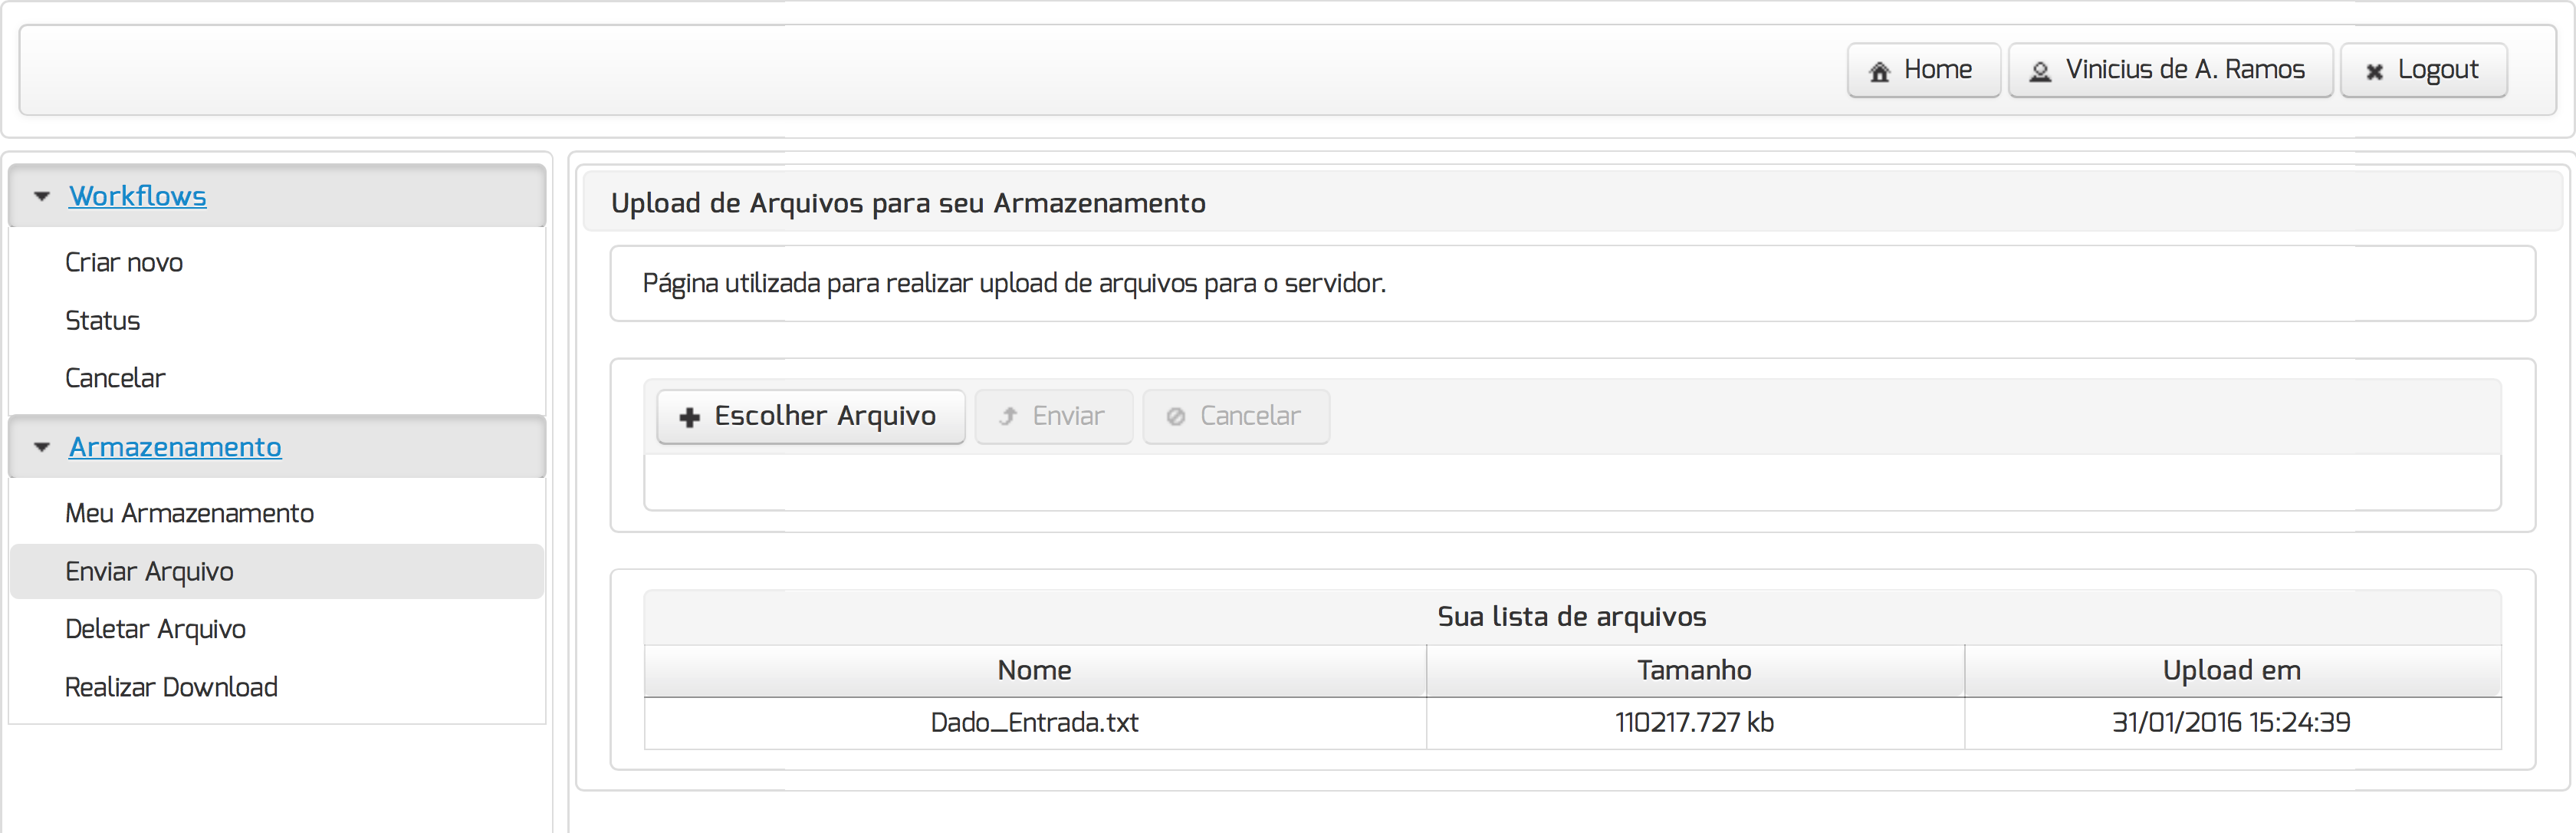
\includegraphics[scale=0.265 ]{tela_upload.png}
	\caption{Tela utilizada para realizar o \textit{upload} de arquivos.}
	\label{fig:tela_upload}
\end{figure}

Nesta implementação, foi definido um armazenamento máximo de 256 \textit{Megabytes} por usuário. Foi desenvolvida uma interface para que usuários possam ter controle de seu armazenamento, apresentada na Figura \ref{fig:tela_armazenamento}.

\begin{figure}[H]
	\centering
	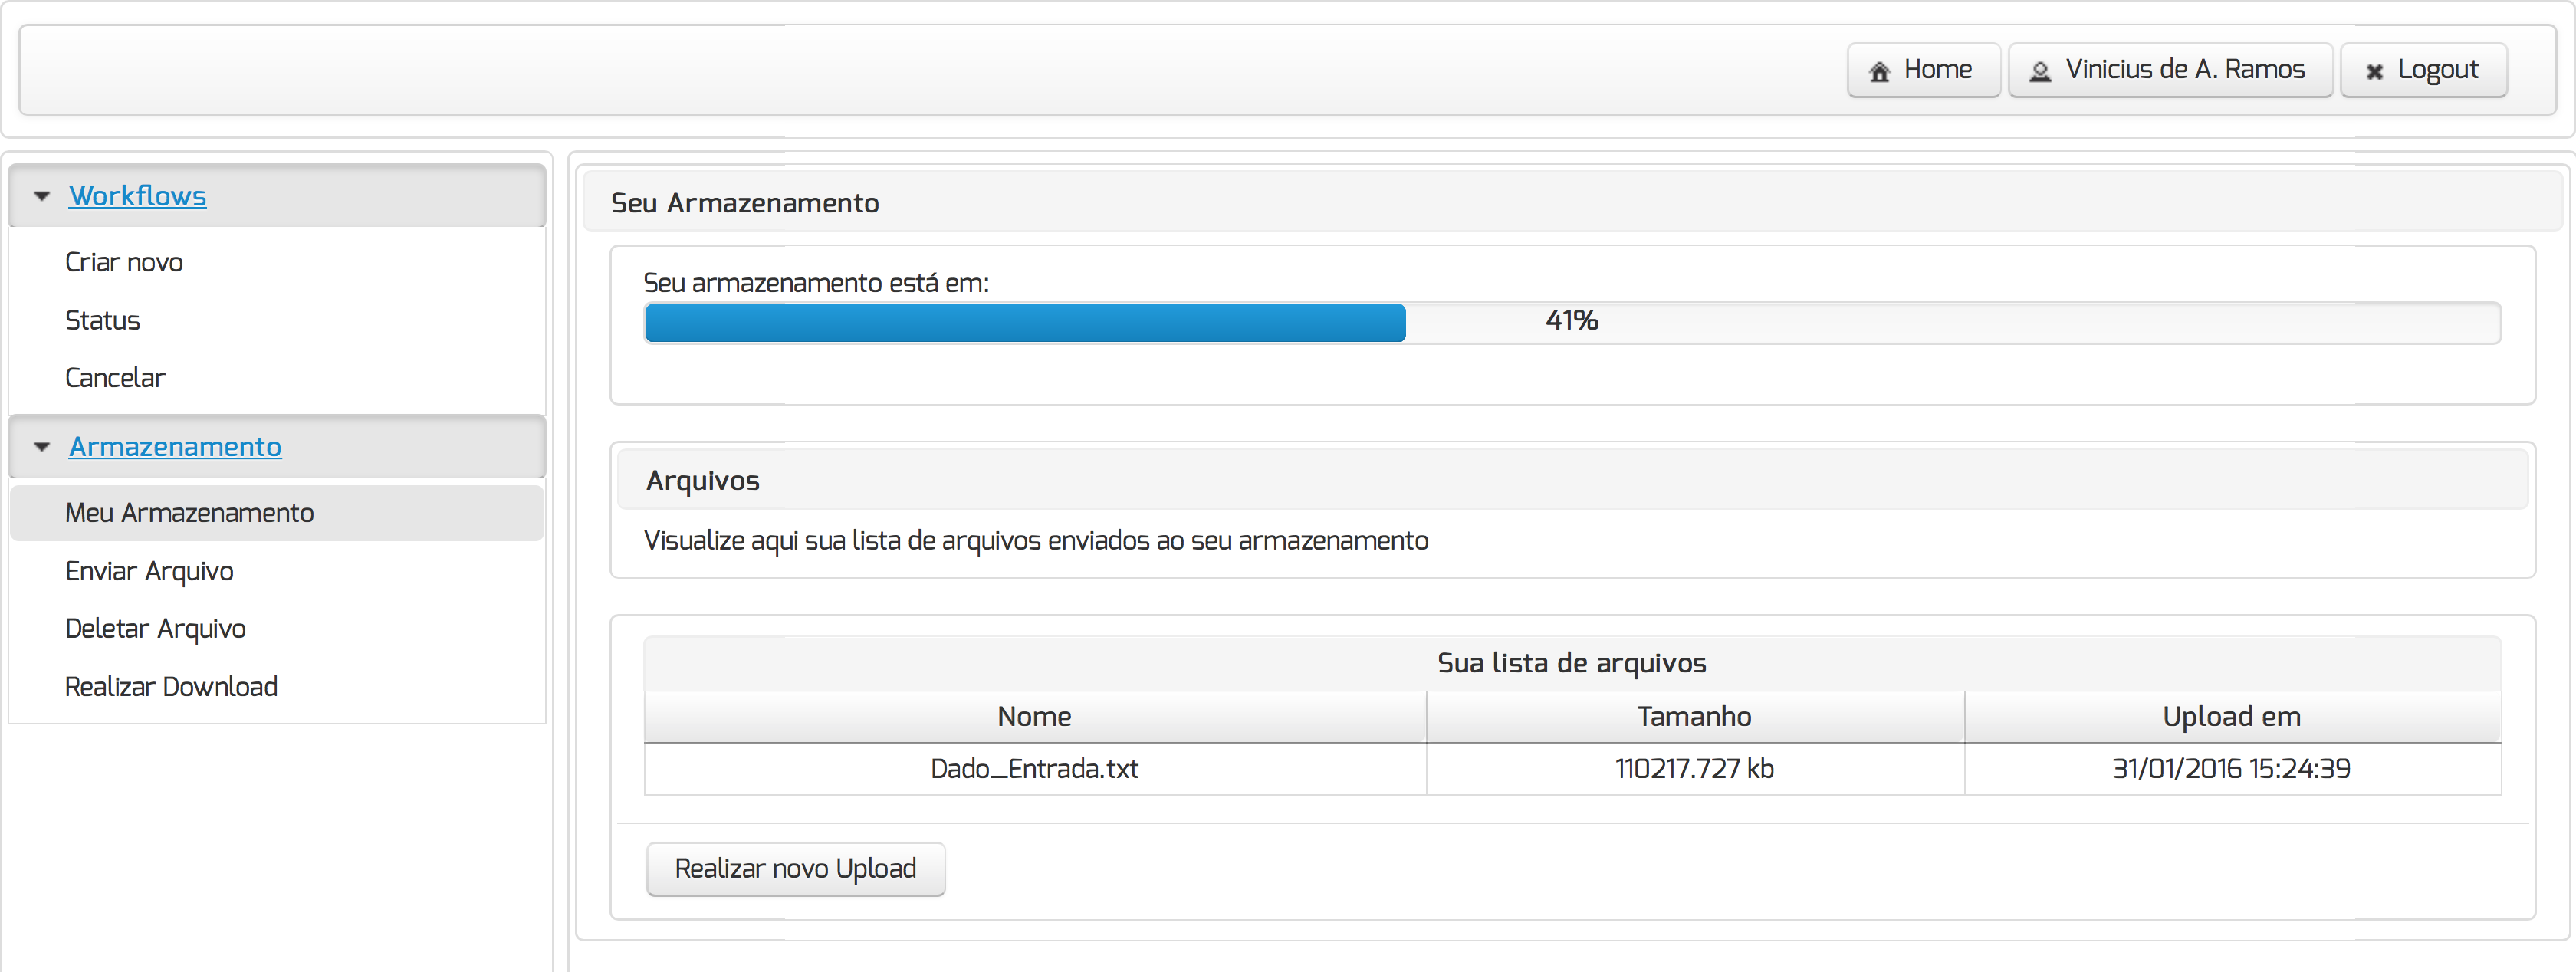
\includegraphics[scale=0.265]{tela_armazenamento.png}
	\caption{Nesta tela usuários controlam seu armazenamento e verificam sua porcentagem.}
	\label{fig:tela_armazenamento}
\end{figure}

Desta forma, as telas apresentadas compõem a camada de visualização do Modelo \textit{MVC}.
